\begin{frame}{Content Overview}
  \footnotesize
    \begin{enumerate}
        \item \textcolor{gray!50}{Motivation, Background, and Objectives}
        \item \colorbox{yellow!70}{\textbf{Addressing the Impossible Trinity of Modeling (ITM)}}
        \item \textcolor{gray!50}{Unified Control-Theoretic Training}
        \item \textcolor{gray!50}{Addressing the Impossible Trinity of Optimal Control (ITOC)}
        \item \textcolor{gray!50}{Conclusions and Future Work}
    \end{enumerate}
\end{frame}

\begin{frame}{\large How does PIROM solve the ITM in small-data regimes?}
    \footnotesize
    \only<1>{
    \begin{figure}
        \centering
        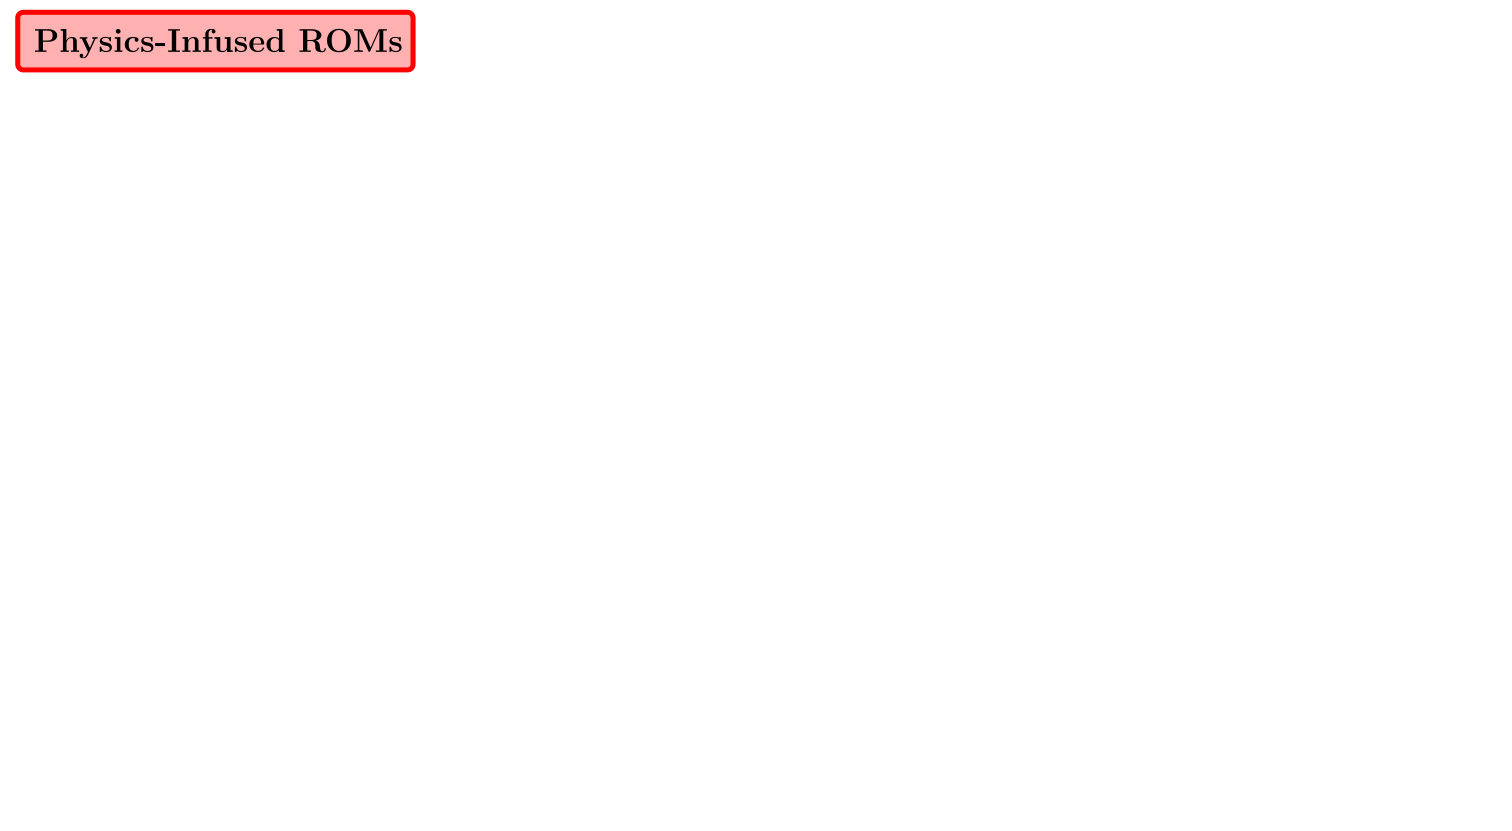
\includegraphics[width=0.9\textwidth]{../figs/sota/physics_infused_1.png}
    \end{figure}}
    \only<2>{
    \begin{figure}
        \centering
        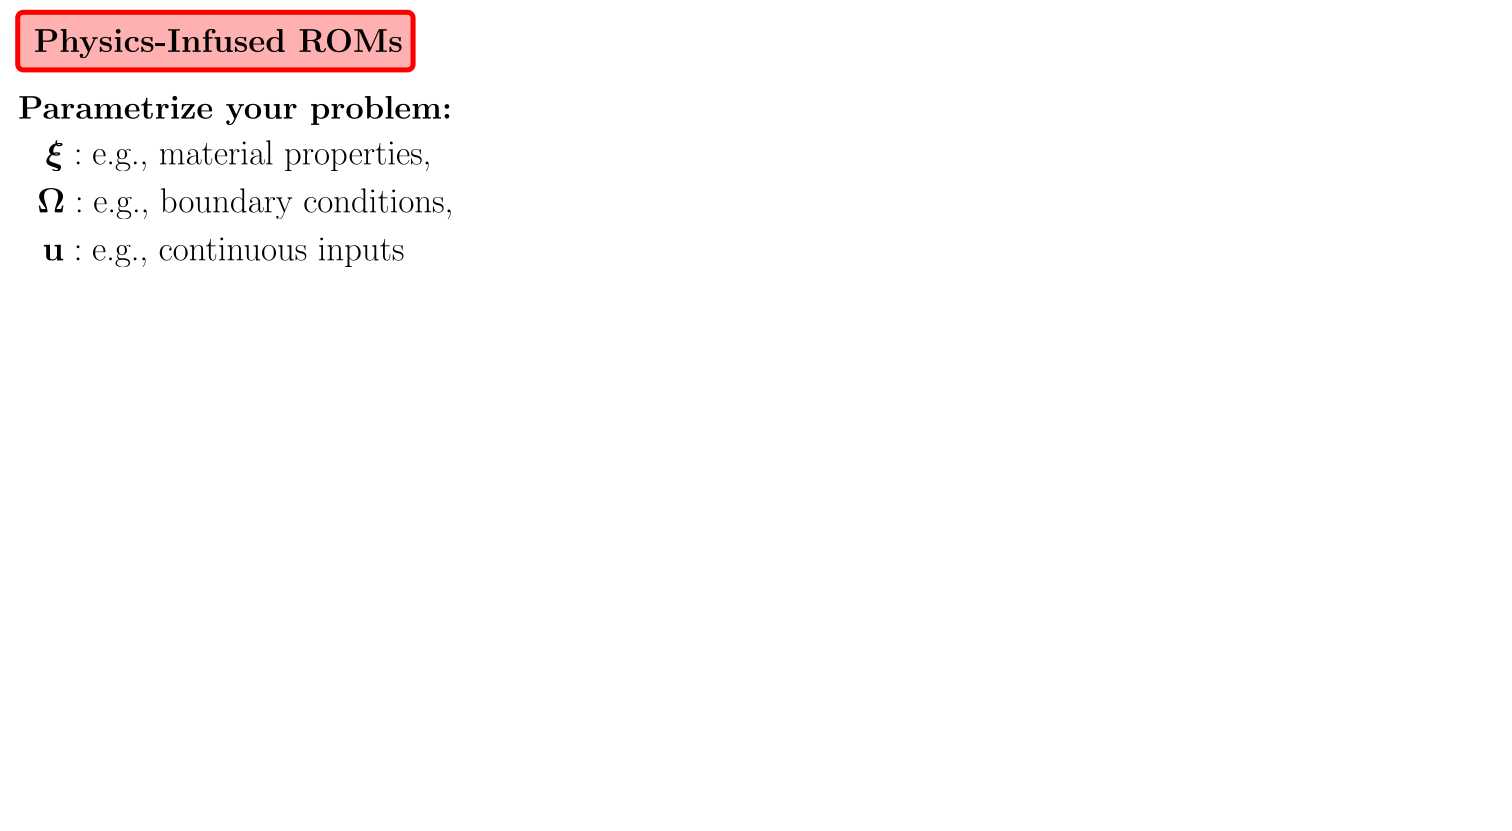
\includegraphics[width=0.9\textwidth]{../figs/sota/physics_infused_2.png}
    \end{figure}}
    \only<3>{
    \begin{figure}
        \centering
        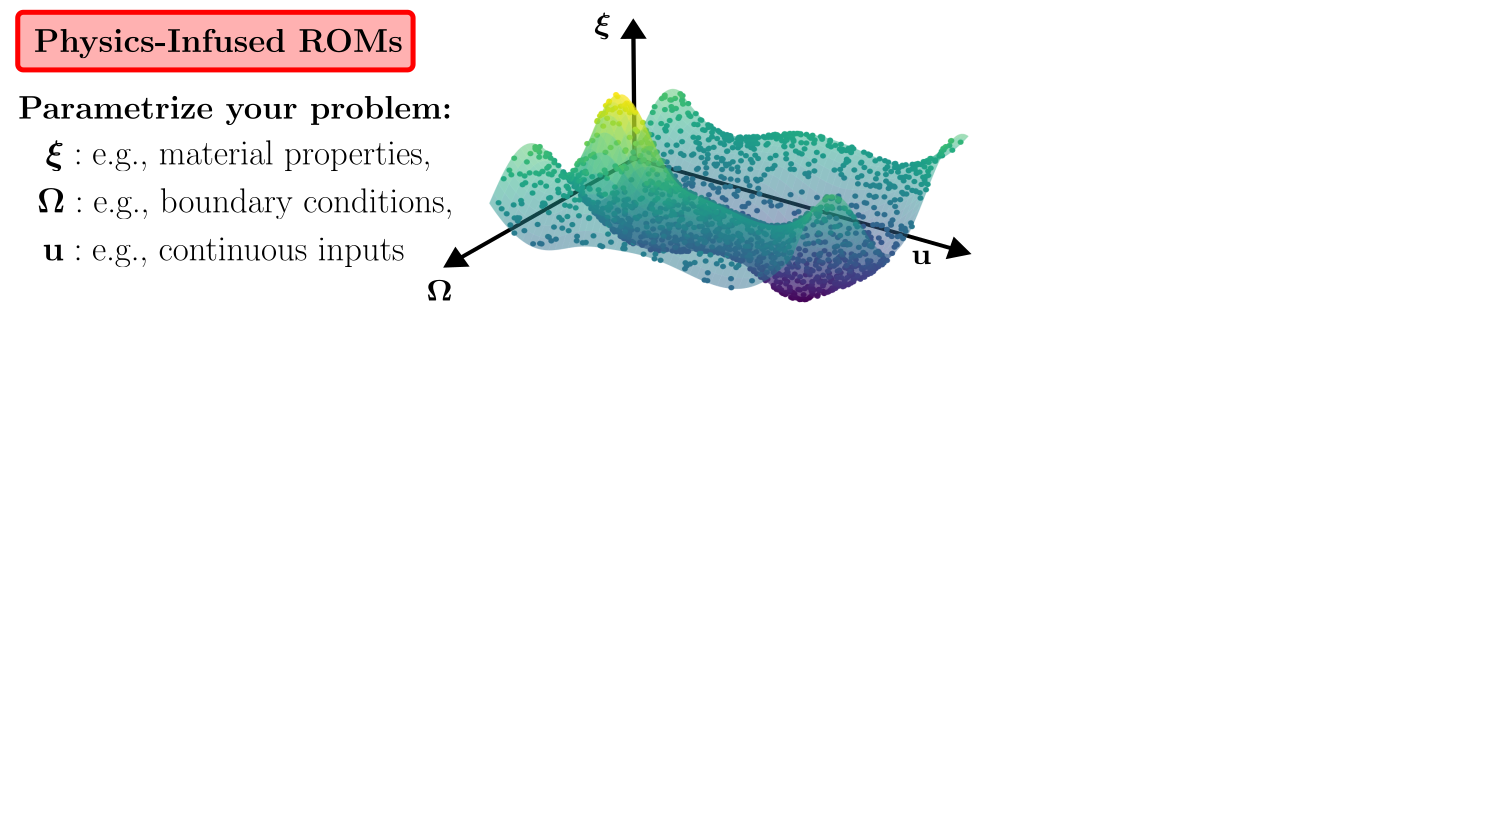
\includegraphics[width=0.9\textwidth]{../figs/sota/physics_infused_3.png}
    \end{figure}}
    \only<4>{
    \begin{figure}
        \centering
        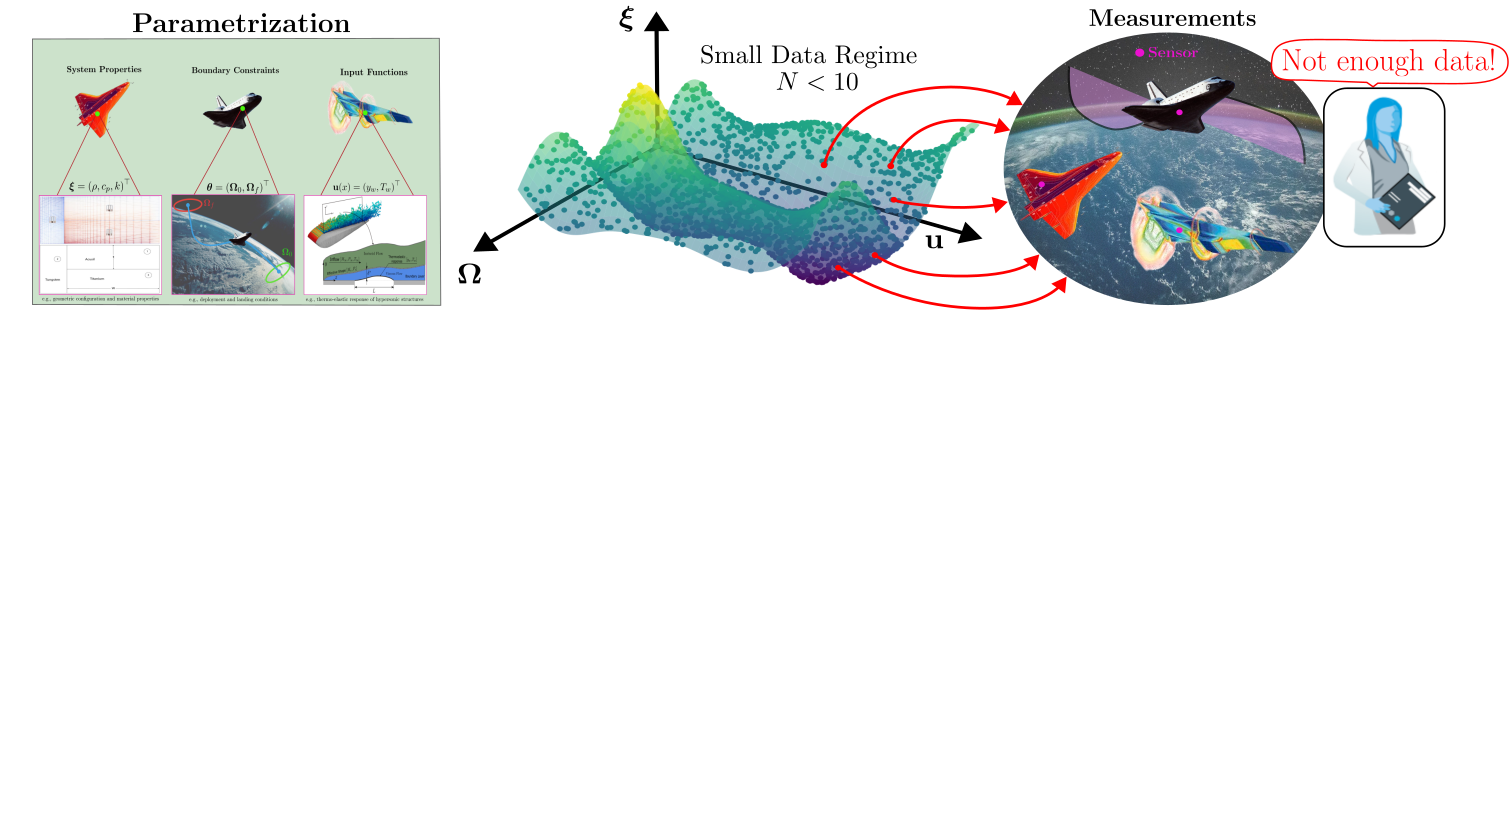
\includegraphics[width=0.9\textwidth]{../figs/sota/physics_infused_4.png}
    \end{figure}}
    \only<5>{
    \begin{figure}
        \centering
        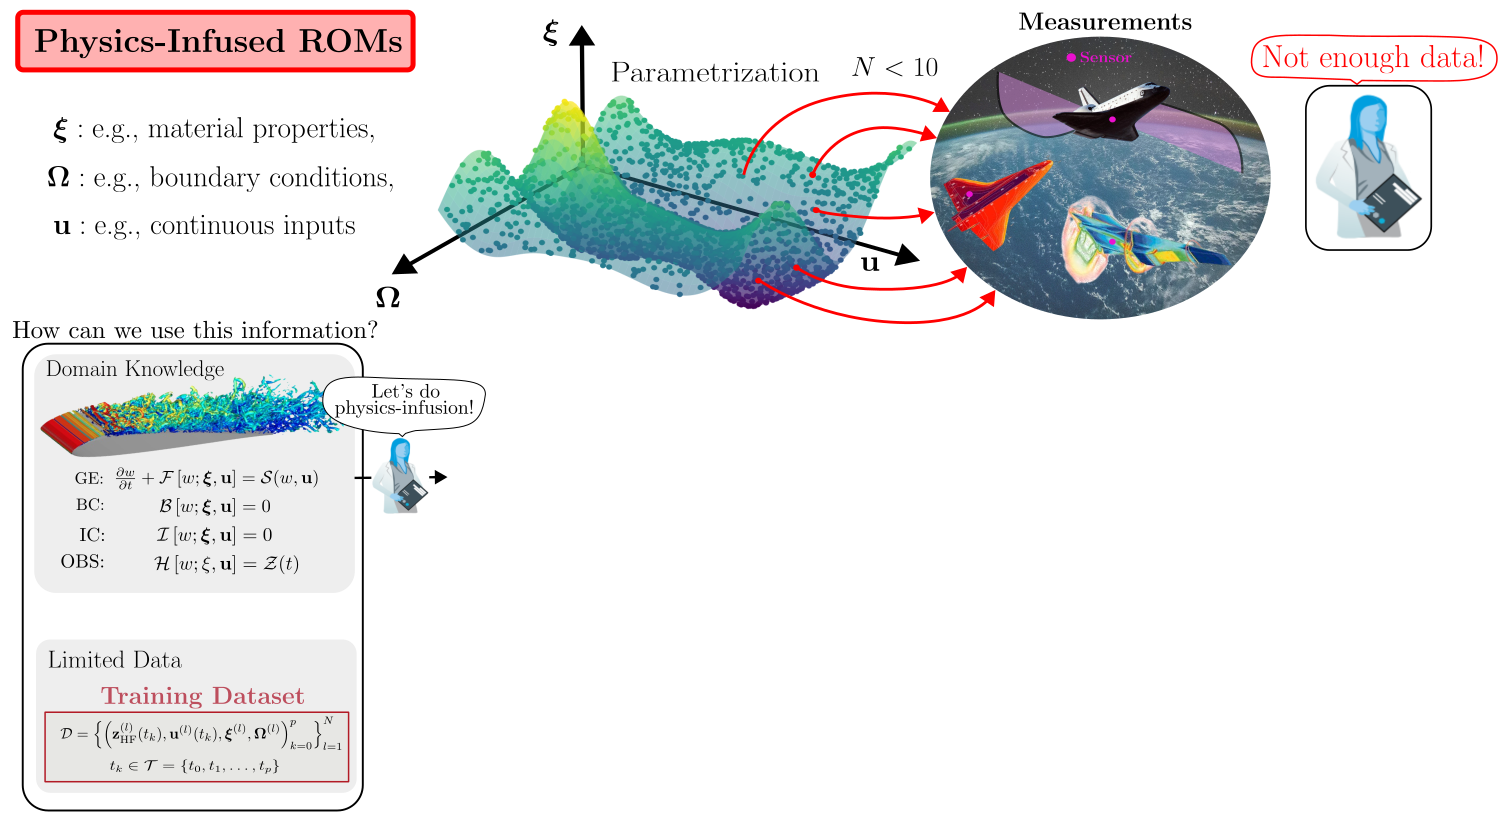
\includegraphics[width=0.9\textwidth]{../figs/sota/physics_infused_5.png}
    \end{figure}}
    \only<6>{
    \begin{figure}
        \centering
        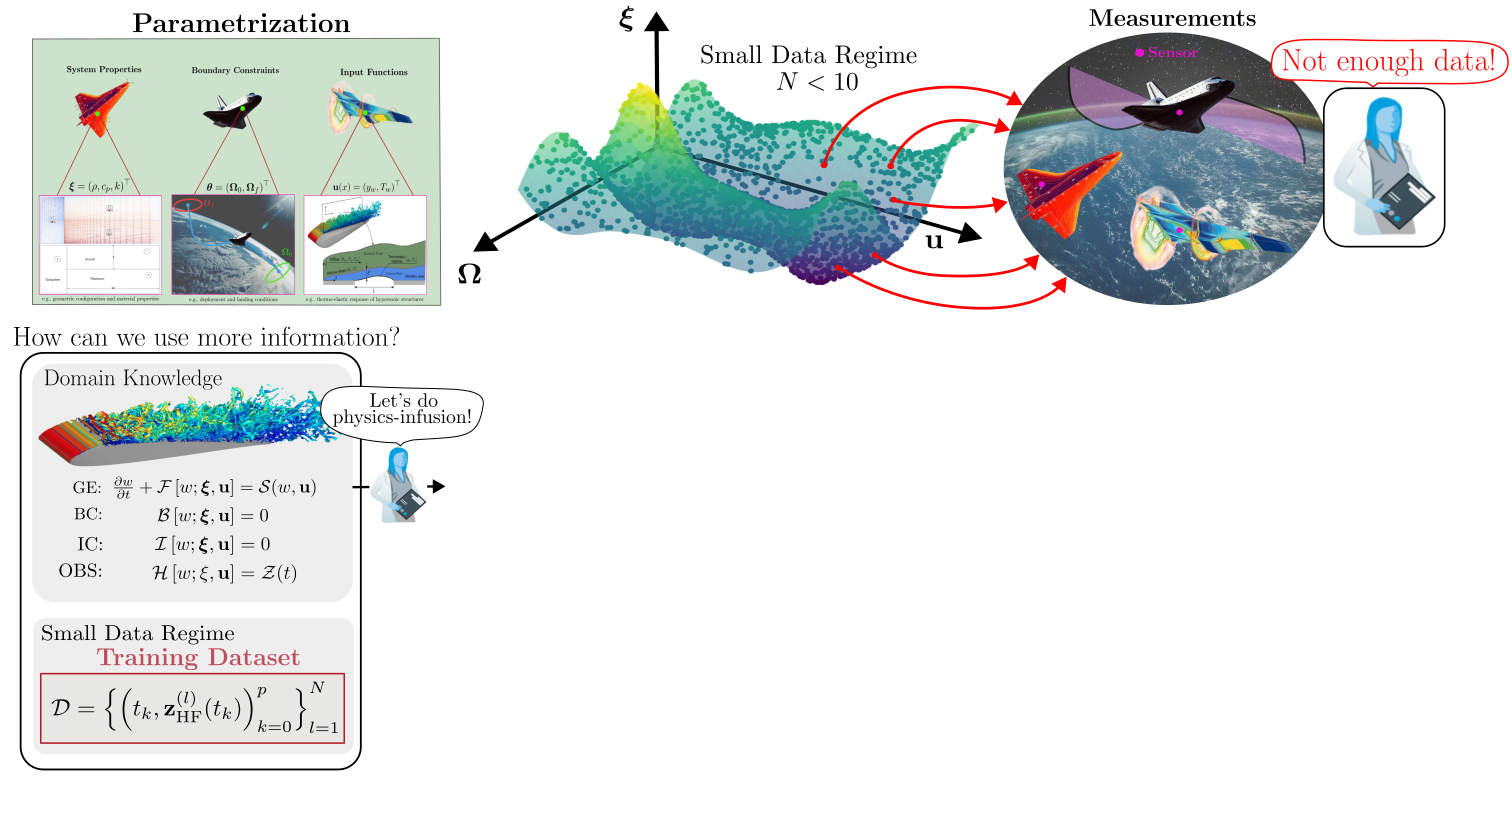
\includegraphics[width=0.9\textwidth]{../figs/sota/physics_infused_6.png}
    \end{figure}}
    \only<7>{
    \begin{figure}
        \centering
        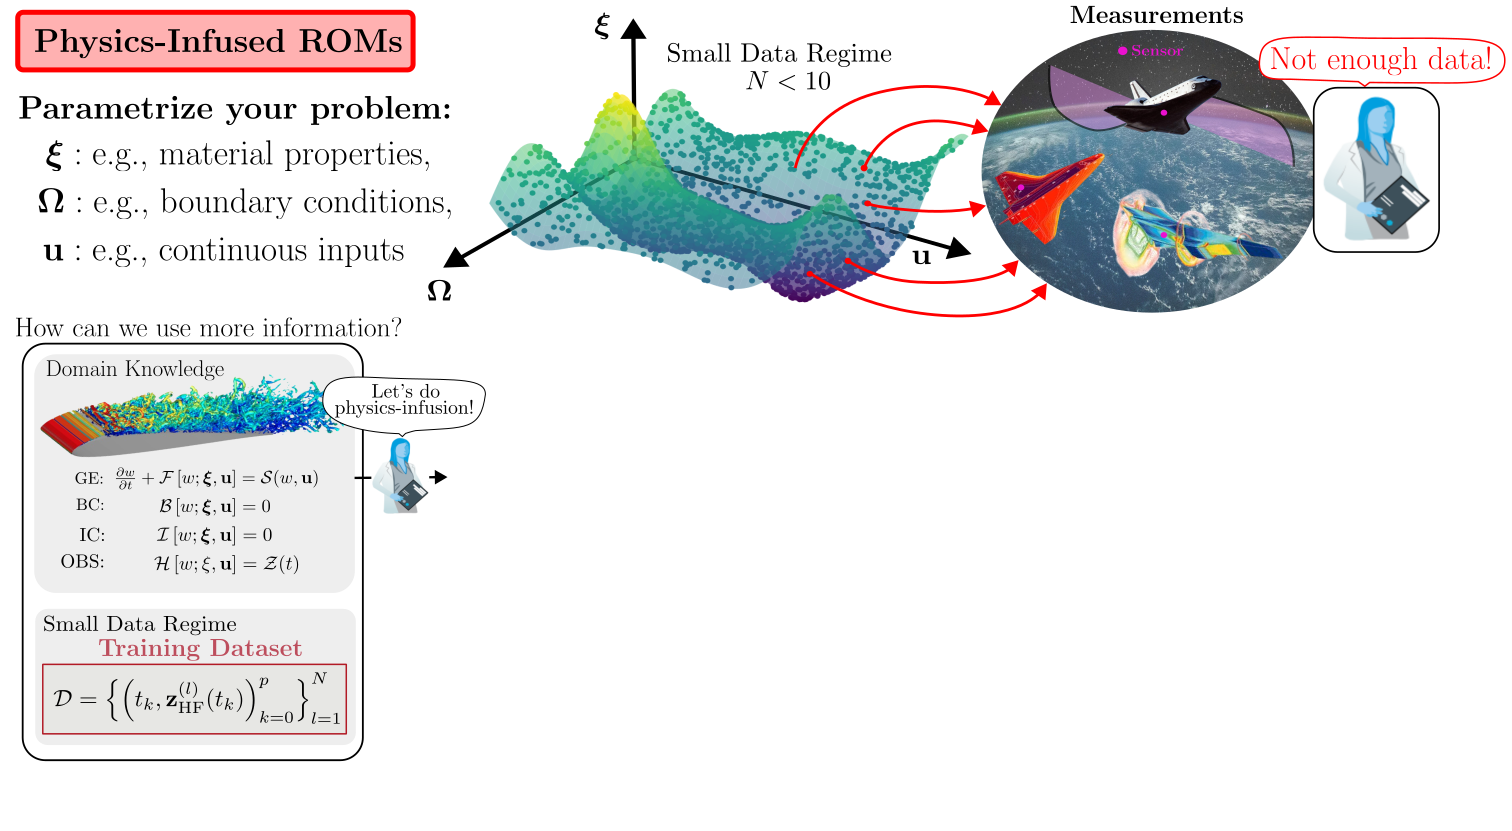
\includegraphics[width=0.9\textwidth]{../figs/sota/physics_infused_7.png}
    \end{figure}}
    \only<8>{
    \begin{figure}
        \centering
        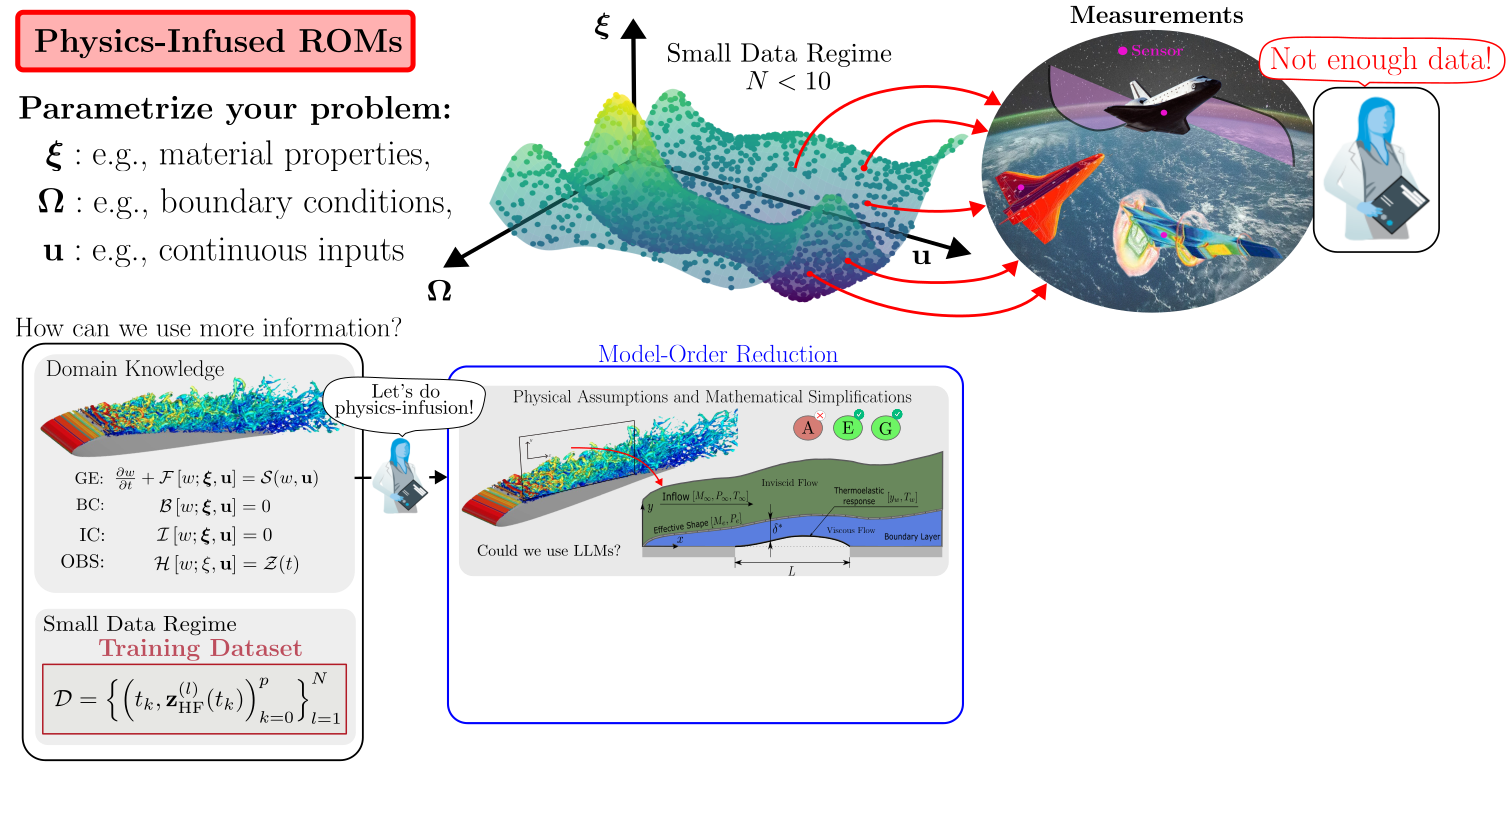
\includegraphics[width=0.9\textwidth]{../figs/sota/physics_infused_8.png}
    \end{figure}}
    \only<9>{
    \begin{figure}
        \centering
        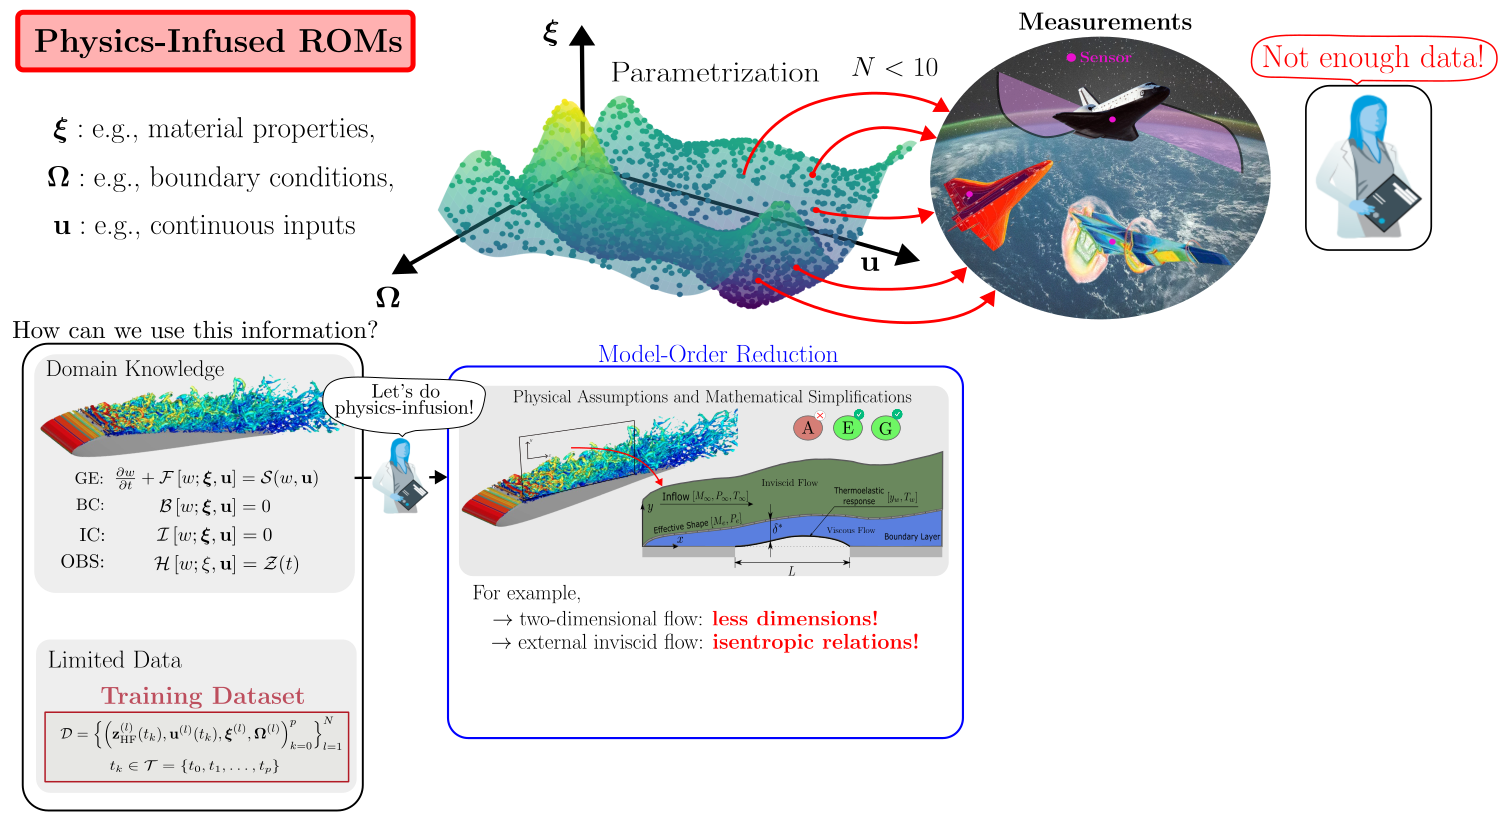
\includegraphics[width=0.9\textwidth]{../figs/sota/physics_infused_9.png}
    \end{figure}}
    \only<10>{
    \begin{figure}
        \centering
        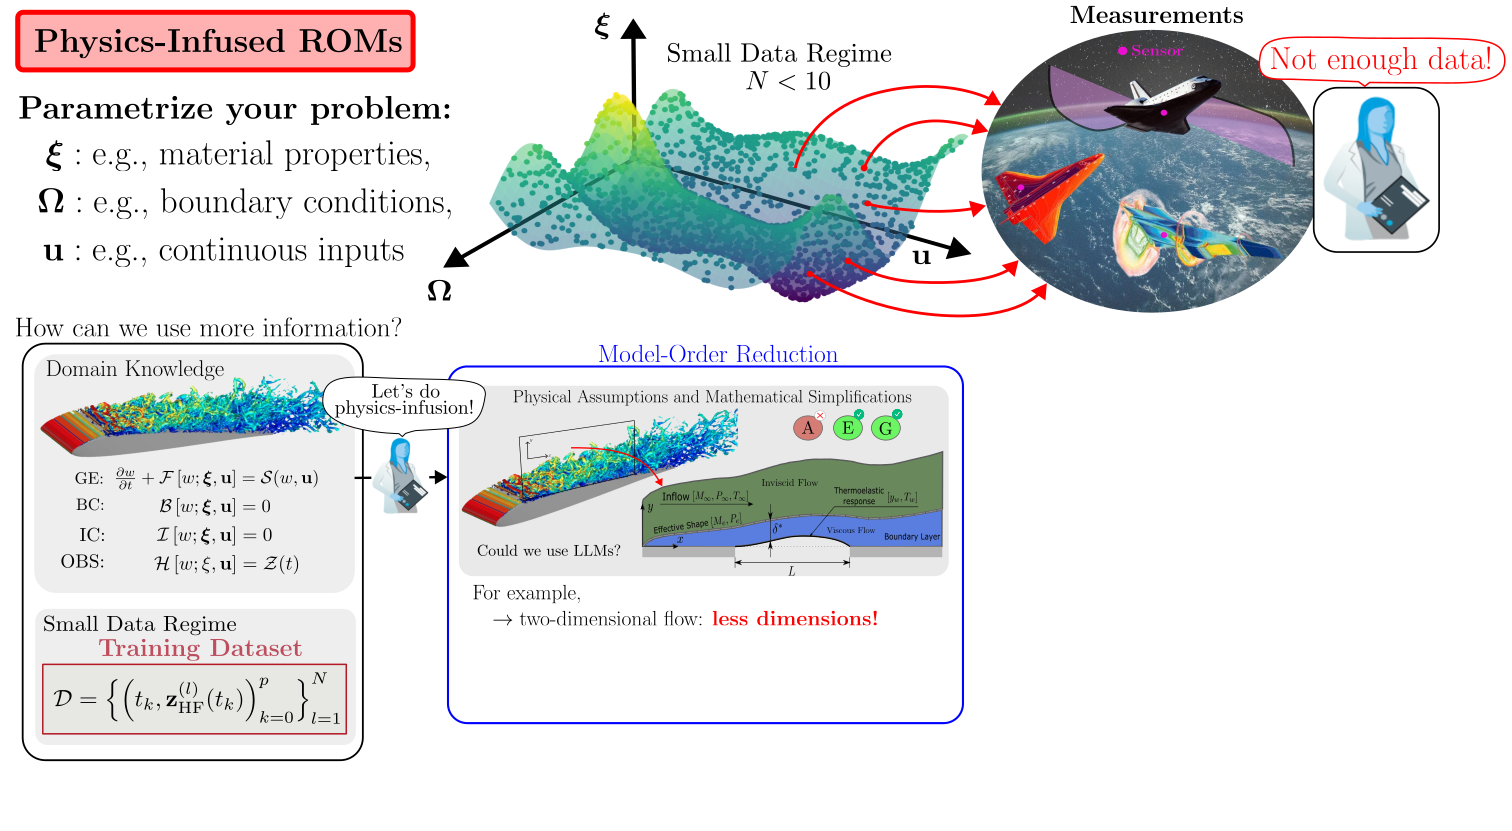
\includegraphics[width=0.9\textwidth]{../figs/sota/physics_infused_10.png}
    \end{figure}}
    \only<11>{
    \begin{figure}
        \centering
        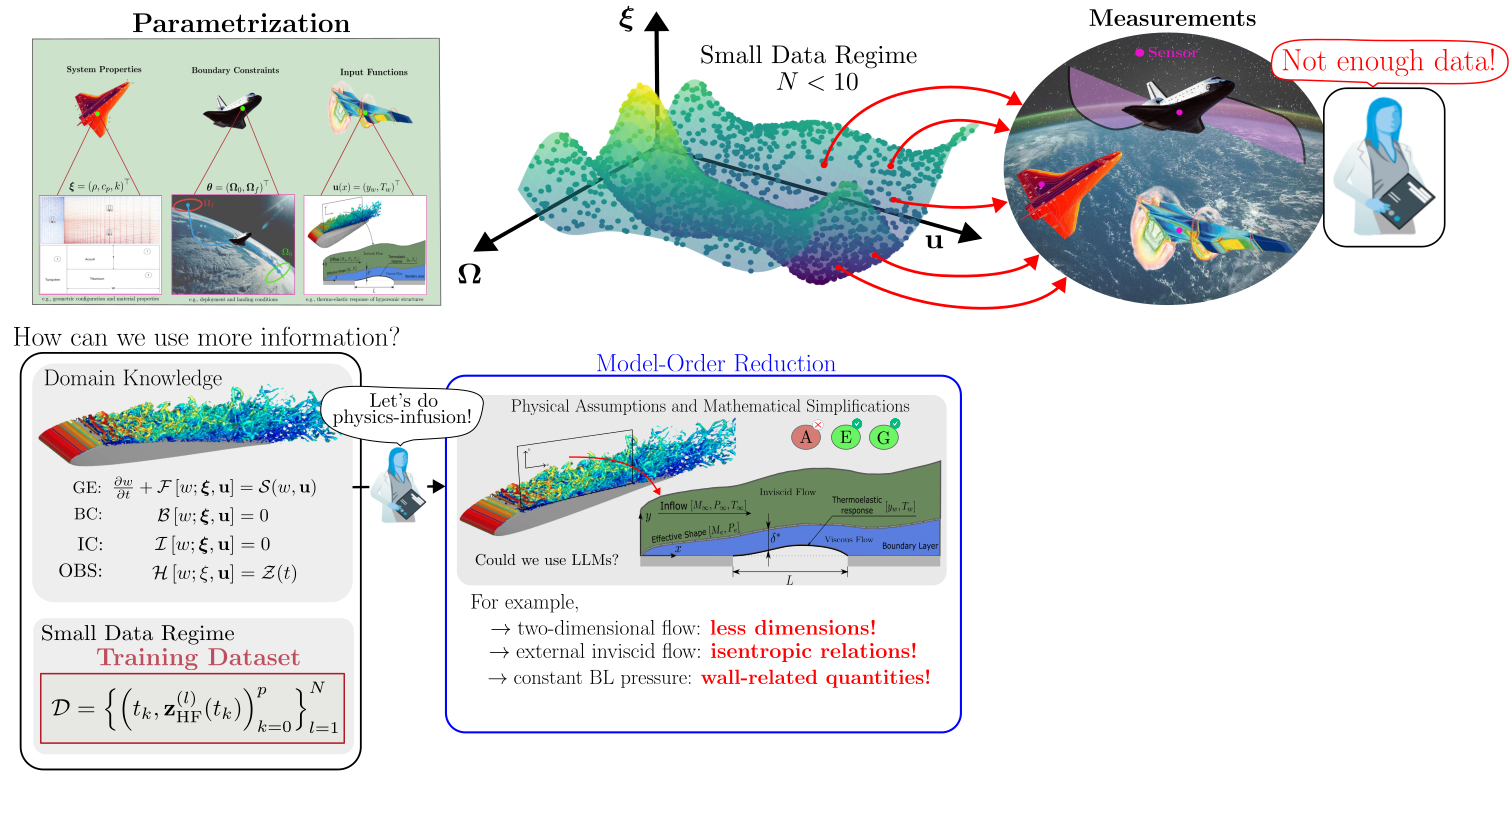
\includegraphics[width=0.9\textwidth]{../figs/sota/physics_infused_11.png}
    \end{figure}}
    \only<12>{
    \begin{figure}
        \centering
        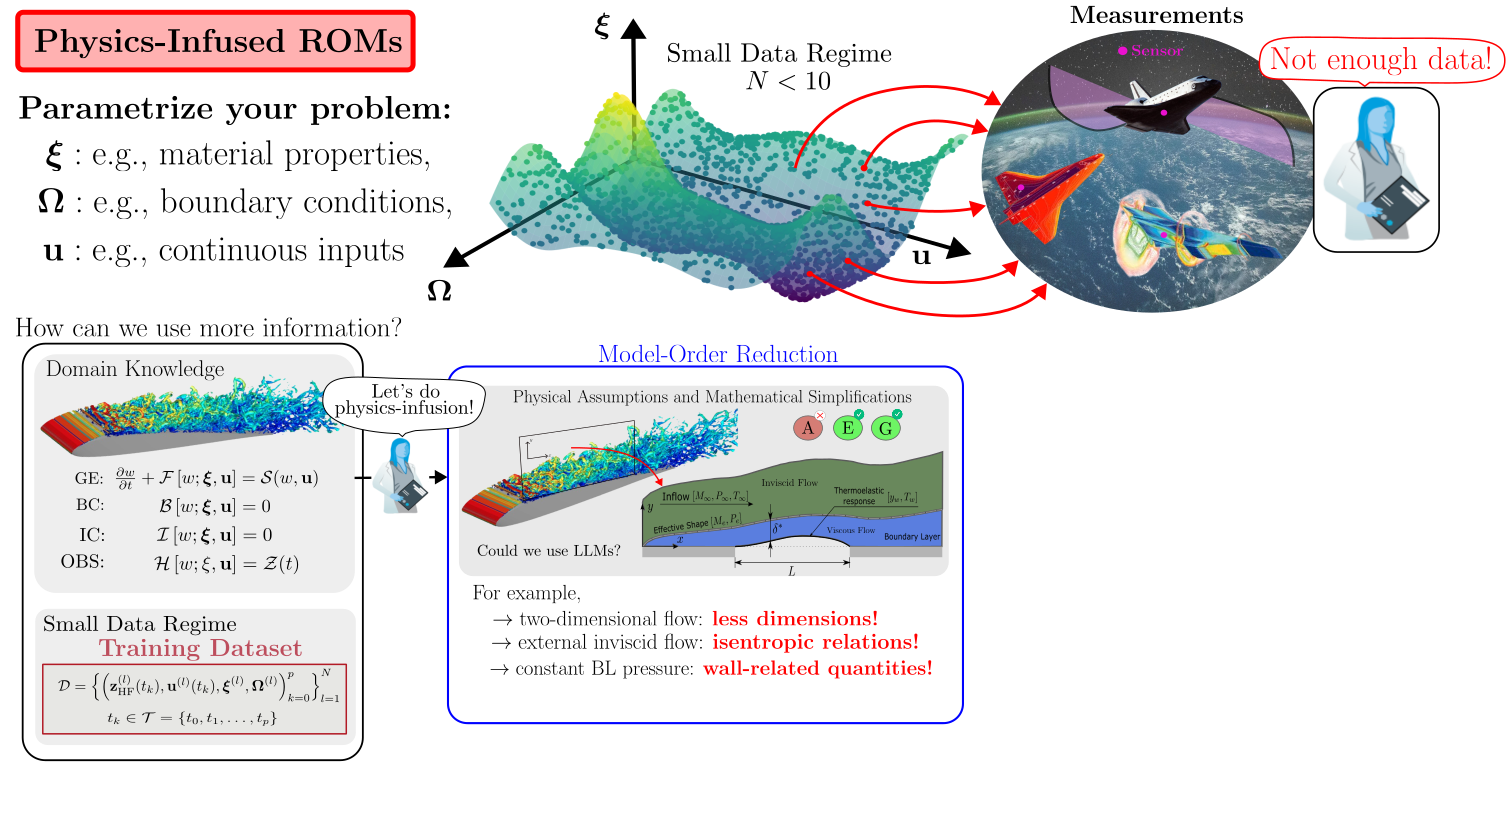
\includegraphics[width=0.9\textwidth]{../figs/sota/physics_infused_12.png}
    \end{figure}}
    \only<13>{
    \begin{figure}
        \centering
        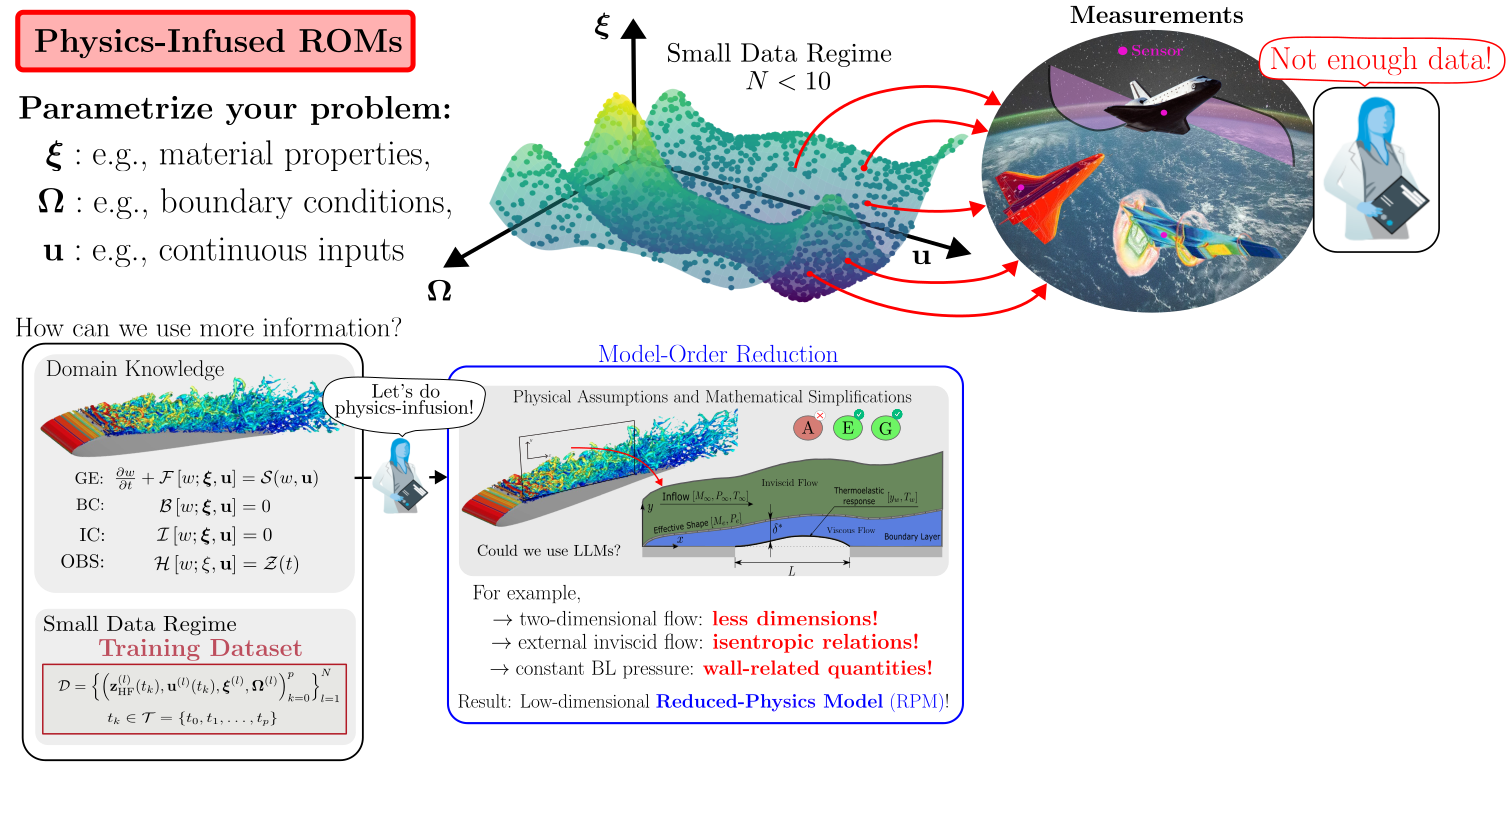
\includegraphics[width=0.9\textwidth]{../figs/sota/physics_infused_13.png}
    \end{figure}}
    \only<14>{
    \begin{figure}
        \centering
        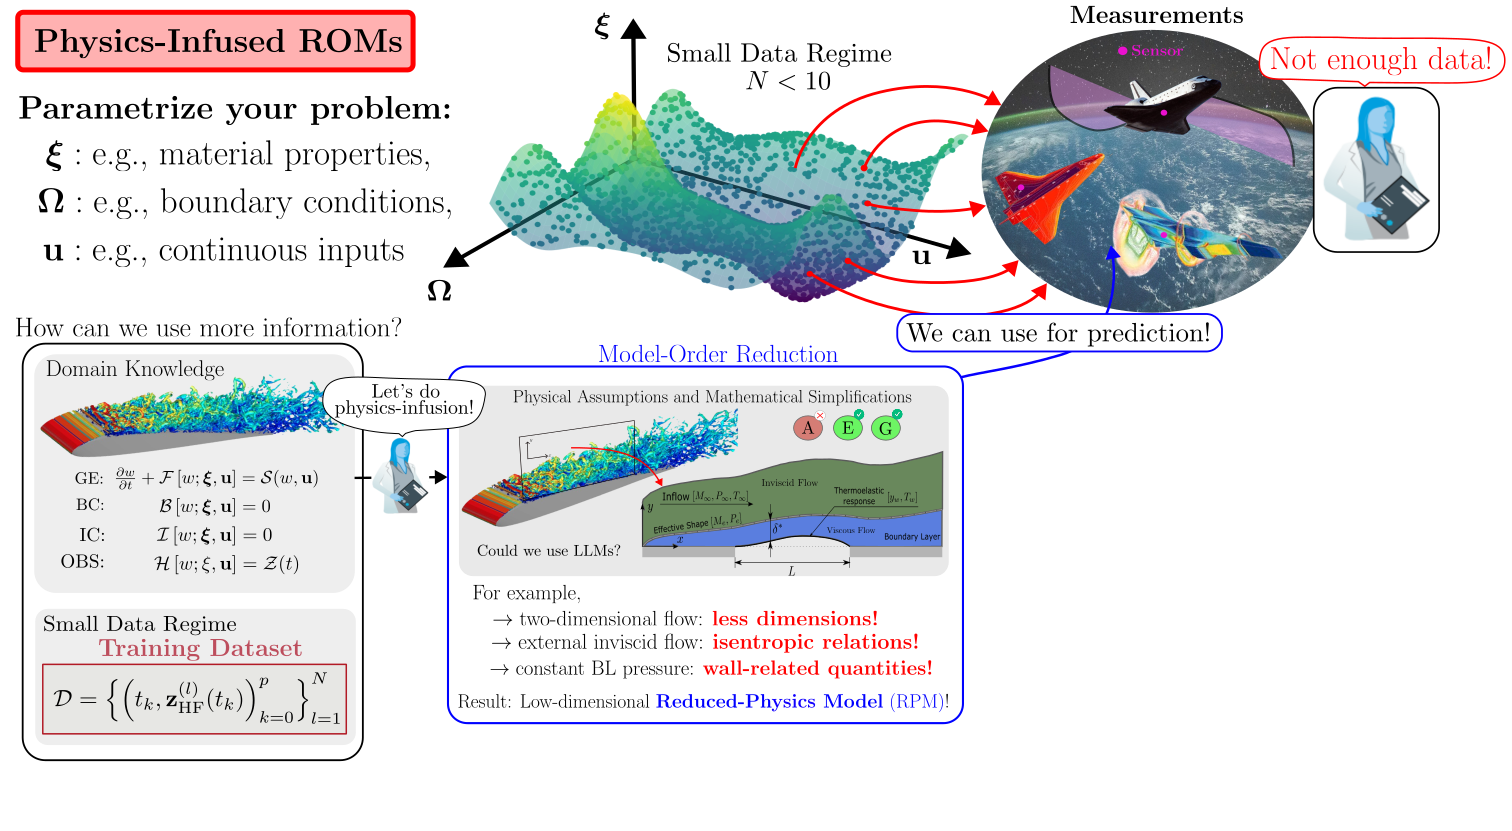
\includegraphics[width=0.9\textwidth]{../figs/sota/physics_infused_14.png}
    \end{figure}}
    \only<15>{
    \begin{figure}
        \centering
        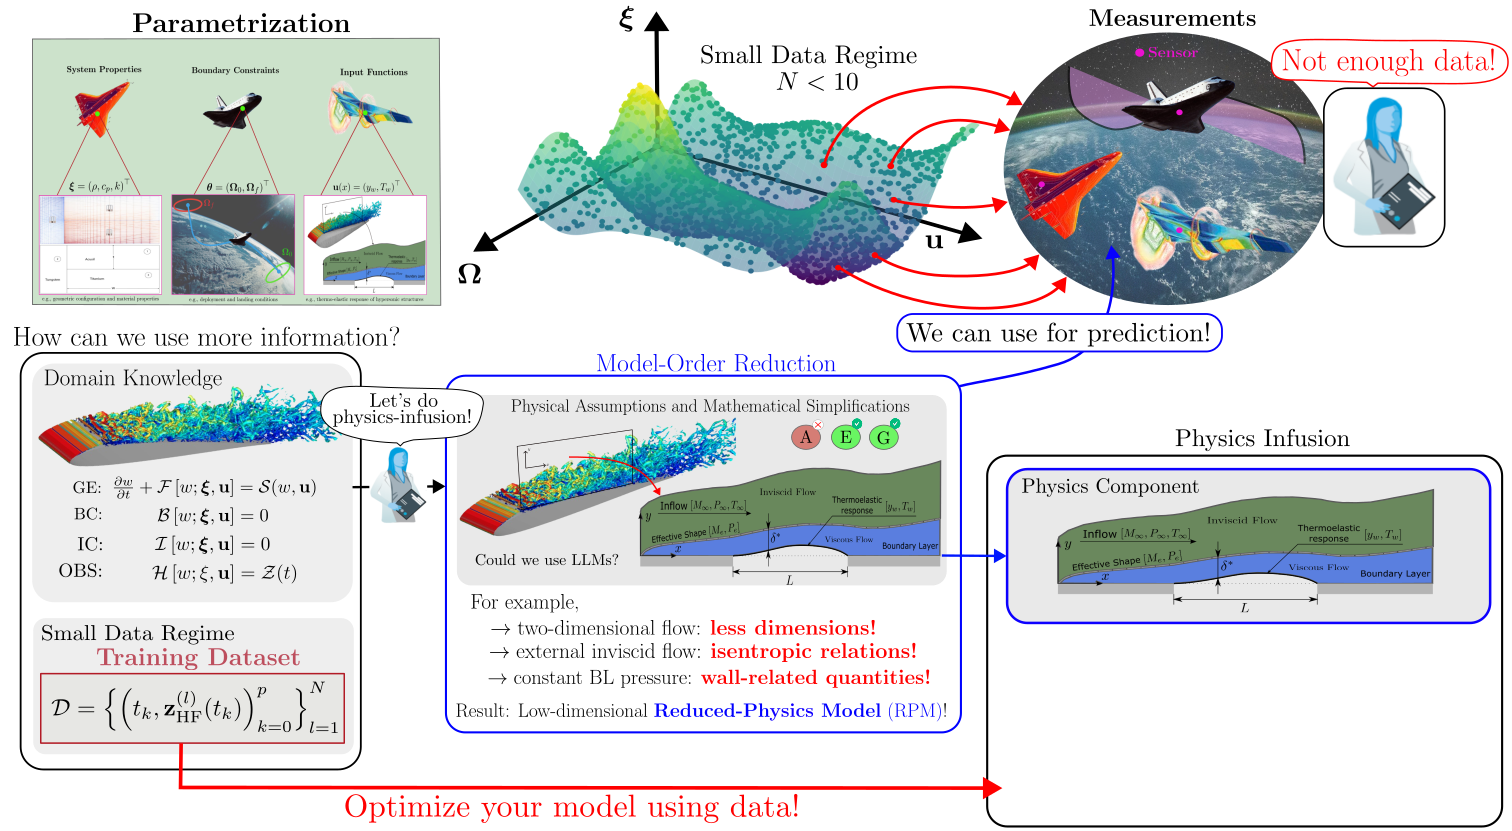
\includegraphics[width=0.9\textwidth]{../figs/sota/physics_infused_15.png}
    \end{figure}}
    \only<16>{
    \begin{figure}
        \centering
        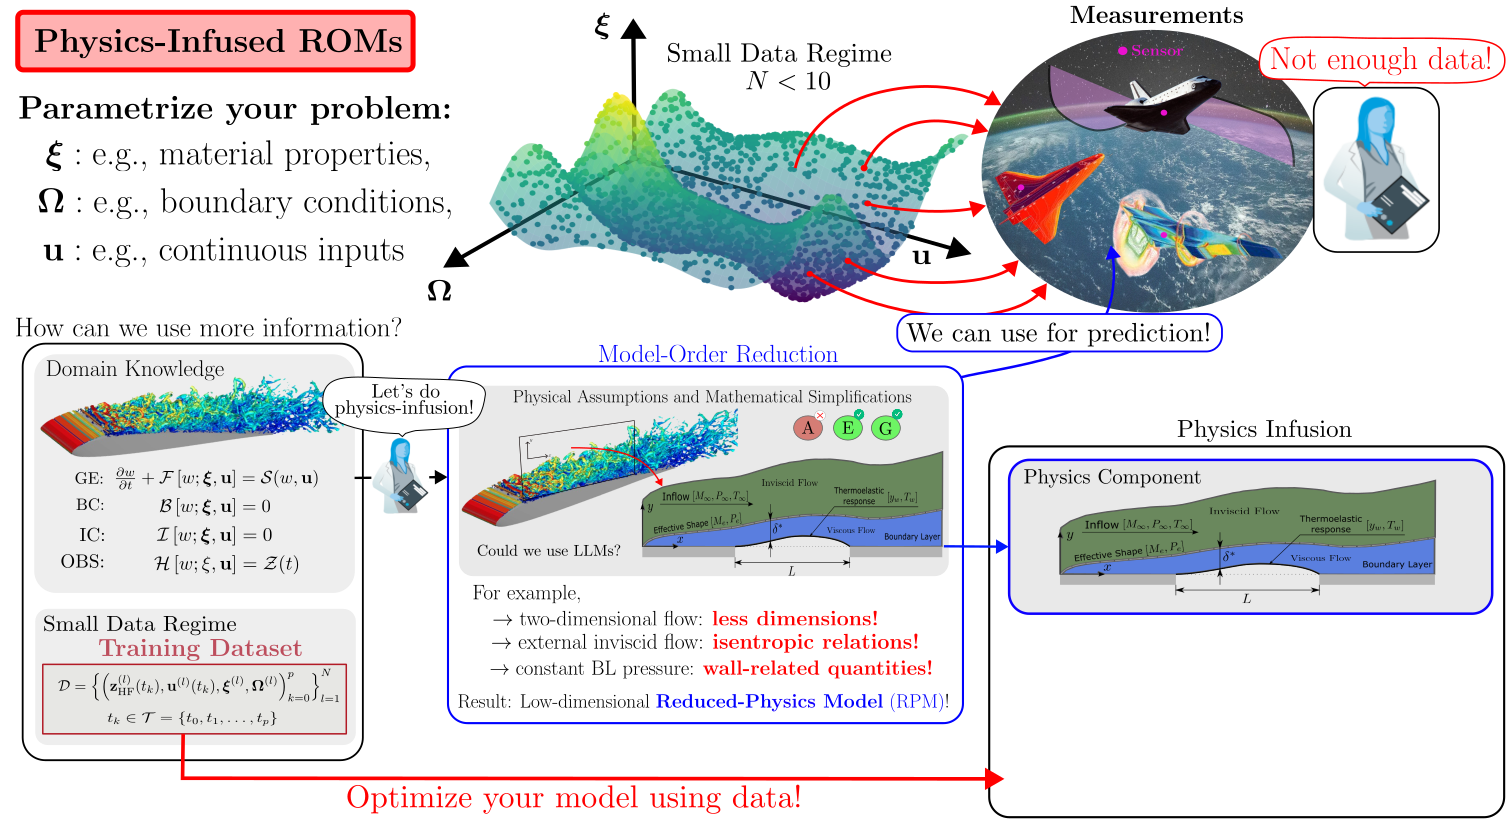
\includegraphics[width=0.9\textwidth]{../figs/sota/physics_infused_16.png}
    \end{figure}}
    \only<17>{
    \begin{figure}
        \centering
        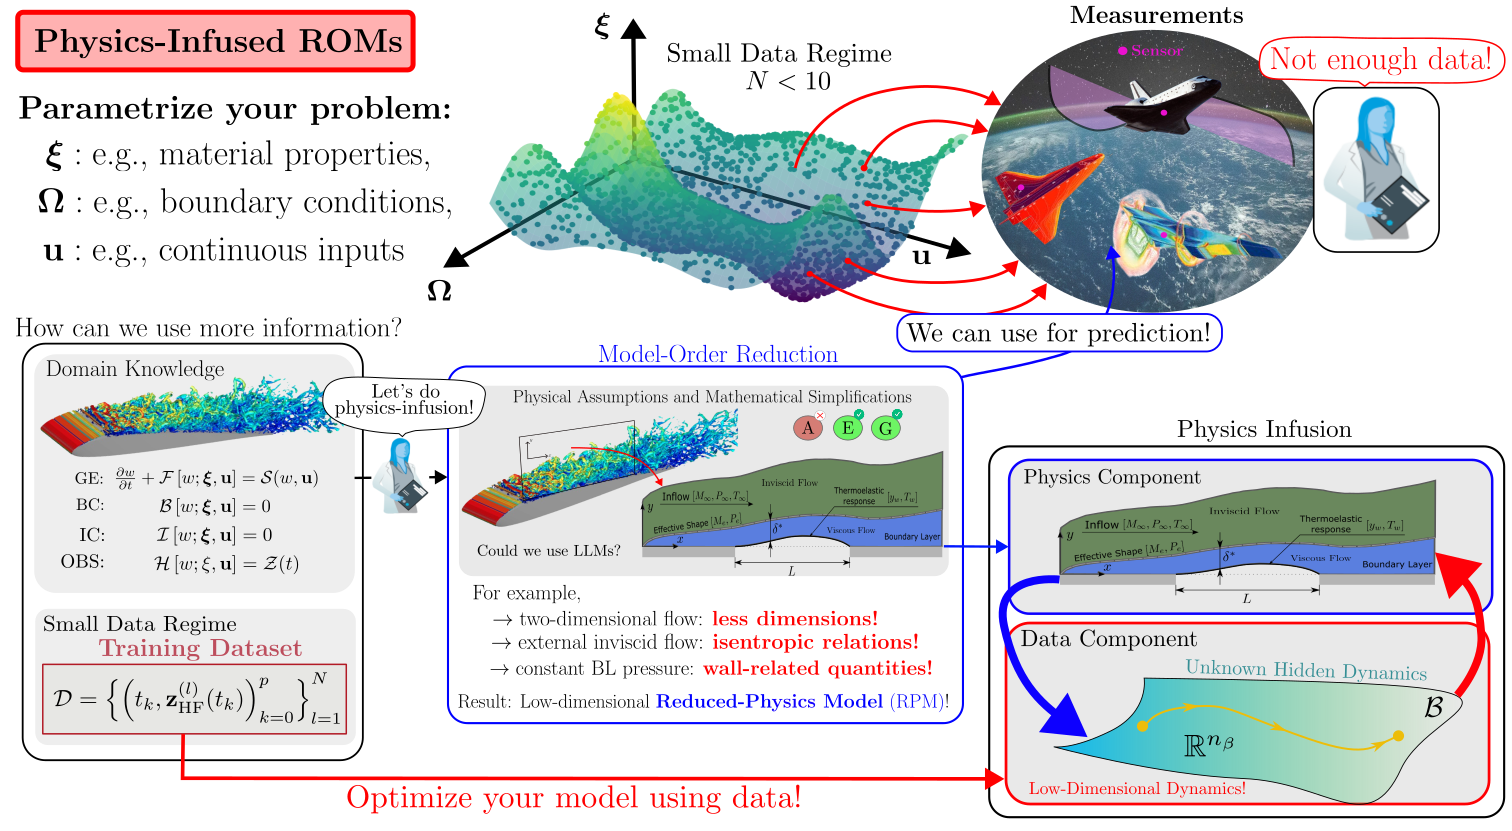
\includegraphics[width=0.9\textwidth]{../figs/sota/physics_infused_17.png}
    \end{figure}}
    \only<18>{
    \begin{figure}
        \centering
        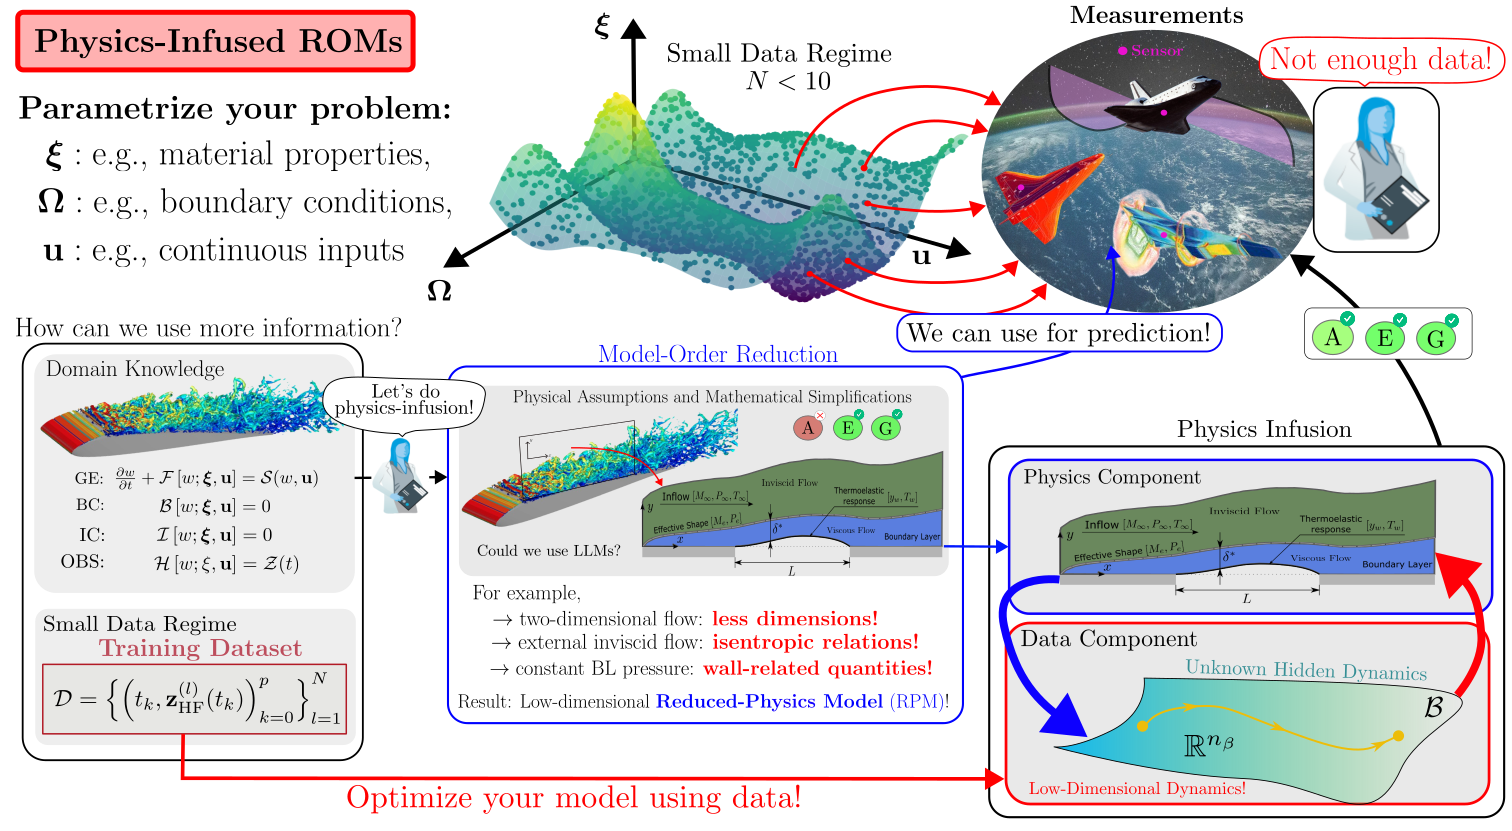
\includegraphics[width=0.9\textwidth]{../figs/sota/physics_infused_18.png}
    \end{figure}}
\end{frame}

\begin{frame}{\large Example: Hypersonic Thermal Protection Systems}
    \footnotesize
    \begin{columns}
        \visible<2->{
        \begin{column}{0.35\textwidth}
            \begin{graybox}{Semi-Discrete FOM}
                For example, FEM yields,
                \vspace*{-0.05in}
                \begin{align*}
                    \dot{\vu} &= \vF\left(\vu;\vp\right)\\
                    \vz_{\text{HF}} &= \vH\left(\vu;\vp\right)\\
                    \vu(t_0) &= \vu_0
                \end{align*}
                \vspace{-0.2in}
                \begin{enumerate}
                    \item<3-> $\vu\in\mathbb{R}^{n_u}$: states $(n_u\gg 1)$
                    \item<4-> $\vp\in\mathbb{R}^{n_p}$: parameters
                    \item<5-> $\vz_{\text{HF}}\in\mathbb{R}^{n_z}$: observable 
                \end{enumerate}
            \end{graybox}
        \end{column}}
        \hspace*{-0.2in}
        \visible<6->{
        \begin{column}{0.70\textwidth}
            \begin{graybox}{Coarse Graining (reduce FOM's complexity)}
                \hspace*{-0.08in}
                \begin{enumerate}
                    \item<7-> State decomposition $\vu = \left[\bvu,\delta\vu\right]^{\top}\in\mathbb{R}^{n_u}$ 
                    \begin{itemize}
                        \item<8-> Observables (e.g., averages) $\bvu\in\mathbb{R}^{n_{\bar{u}}}$
                        \item<9-> Un-observables (e.g., deviations) $\delta\vu\in\mathbb{R}^{n_{\delta u}}$ $\left(n_{\delta u}\gg n_{\bar{u}}\right)$
                    \end{itemize}
                    \item<10-> Projection operator $\cP:\cH_{n_u}\to\cH_{n_{\bar{u}}}\subset\cH_{n_u}$, e.g.,
                    \vspace*{-0.1in}
                    \begin{equation*}
                        \cP: \cG\left(\vu\right)\rightarrow \bar{\cG}\left(\bvu\right)\rightarrow\text{cheaper to evaluate!}
                        \vspace*{-0.1in}
                    \end{equation*}
                    \item<11-> Complement operator $\cQ = \cI - \cP$
                \end{enumerate}
                \vspace{-0.1in}
                \visible<12->{
                \begin{figure}
                    \centering
                    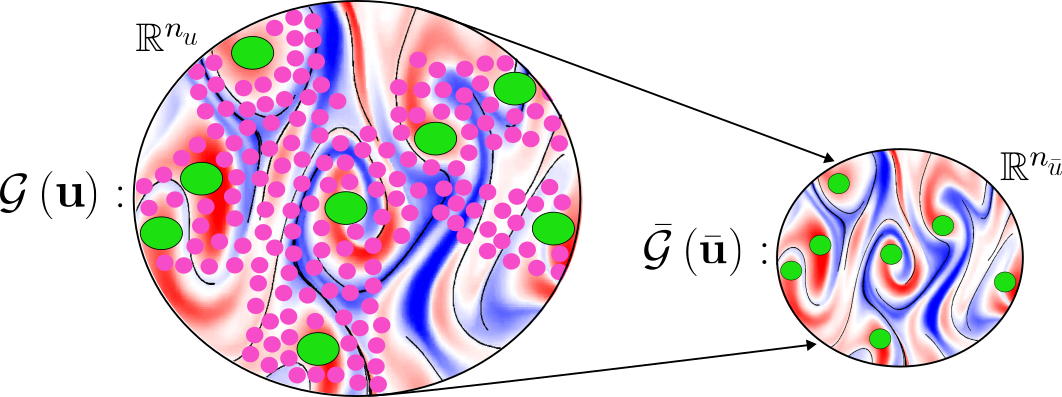
\includegraphics[width=0.65\textwidth]{../figs/pirom/coarse_graining.png}
                \end{figure}}
                \vspace*{-0.1in}
            \end{graybox}
        \end{column}}
    \end{columns}
\end{frame}

\begin{frame}{Addressing the ITM: Coarse Graining}
    \footnotesize
    \visible<1->{
        \textbf{For example}, we can apply \textbf{coarse-graining} principles to \textbf{hypersonic TPS} models {\tiny [2,3]},}
    \vspace*{-0.1in}
    \begin{columns}
        \visible<1->{
        \begin{column}{0.55\textwidth}
            \only<1>{
                \begin{figure}
                    \centering
                    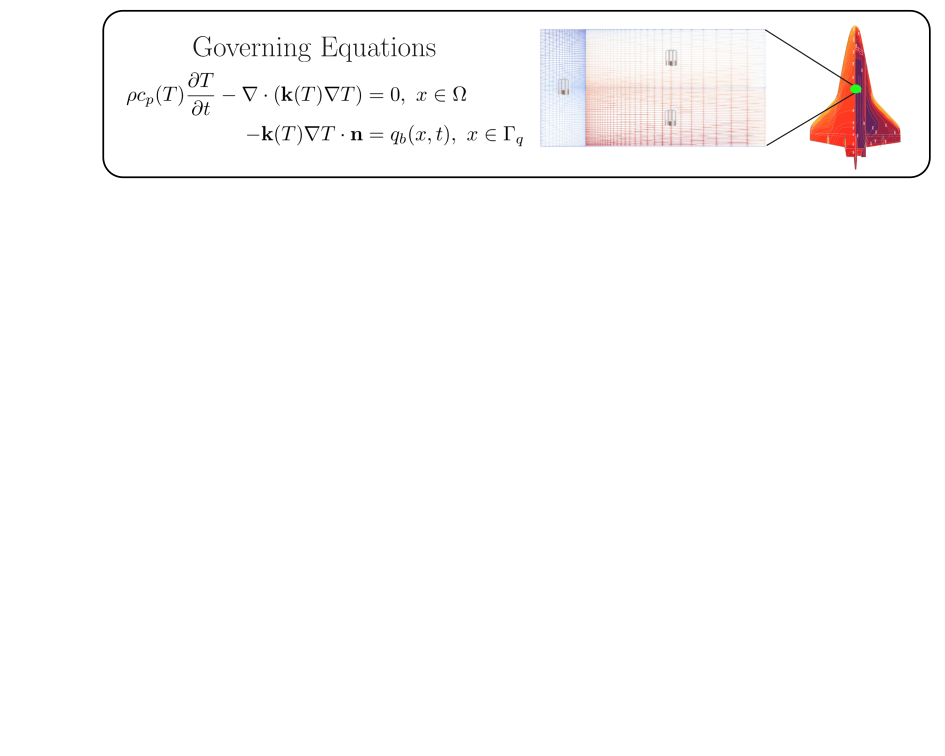
\includegraphics[width=0.85\textwidth]{../figs/pirom/coarse_graining_tps_left_1.png}
                \end{figure}}
            \only<2>{
                \begin{figure}
                    \centering
                    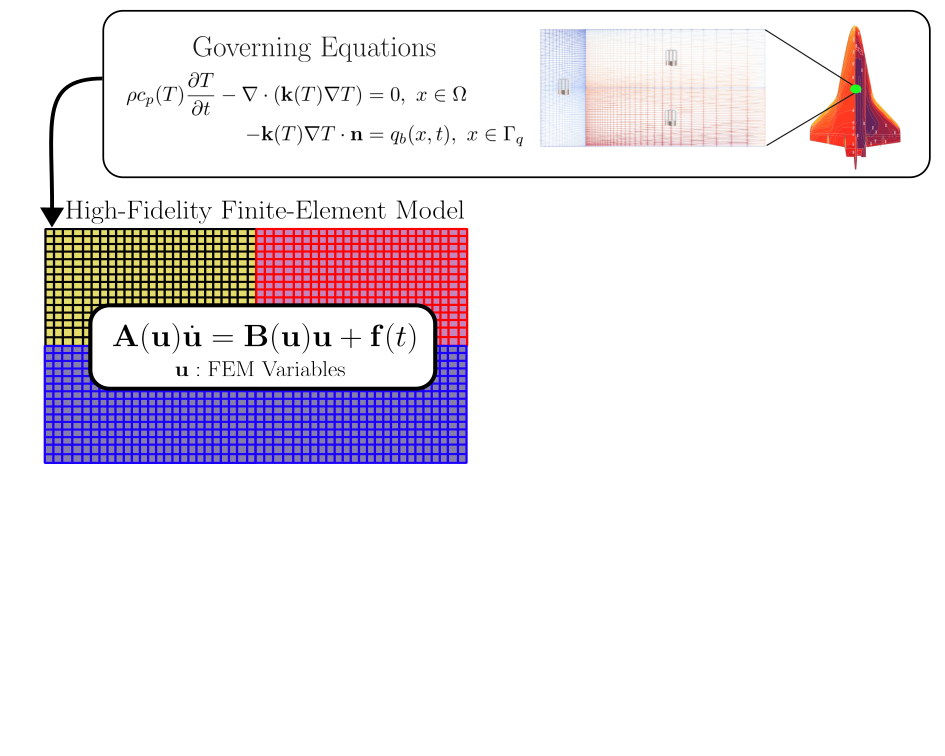
\includegraphics[width=0.85\textwidth]{../figs/pirom/coarse_graining_tps_left_2.png}
                \end{figure}}
            \only<3>{
                \begin{figure}
                    \centering
                    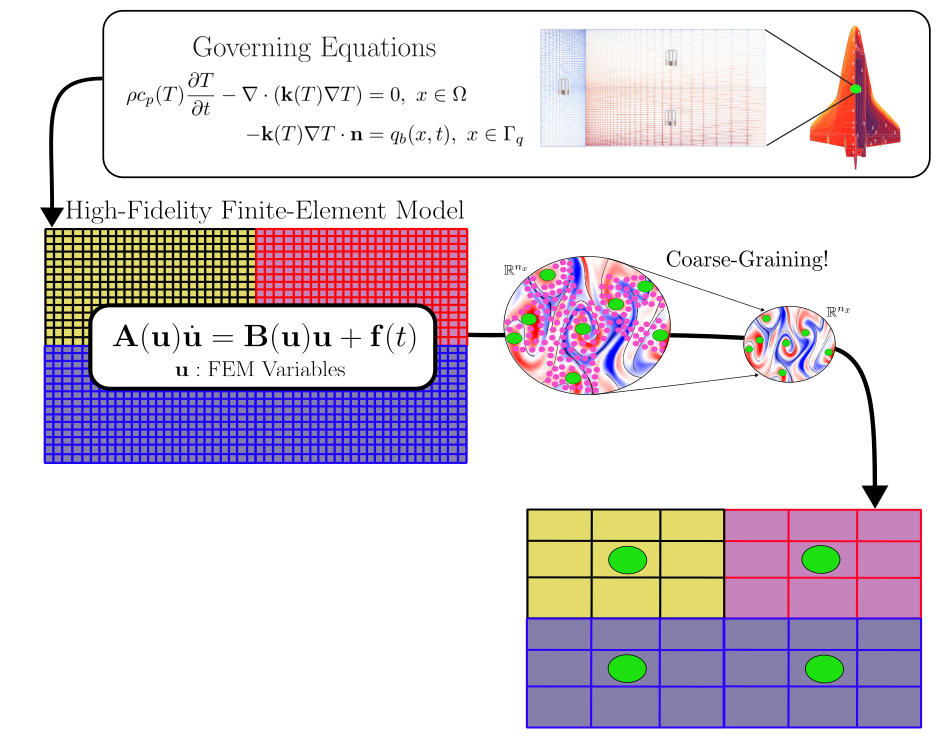
\includegraphics[width=0.85\textwidth]{../figs/pirom/coarse_graining_tps_left_3.png}
                \end{figure}}
            \only<4->{
                \begin{figure}
                    \centering
                    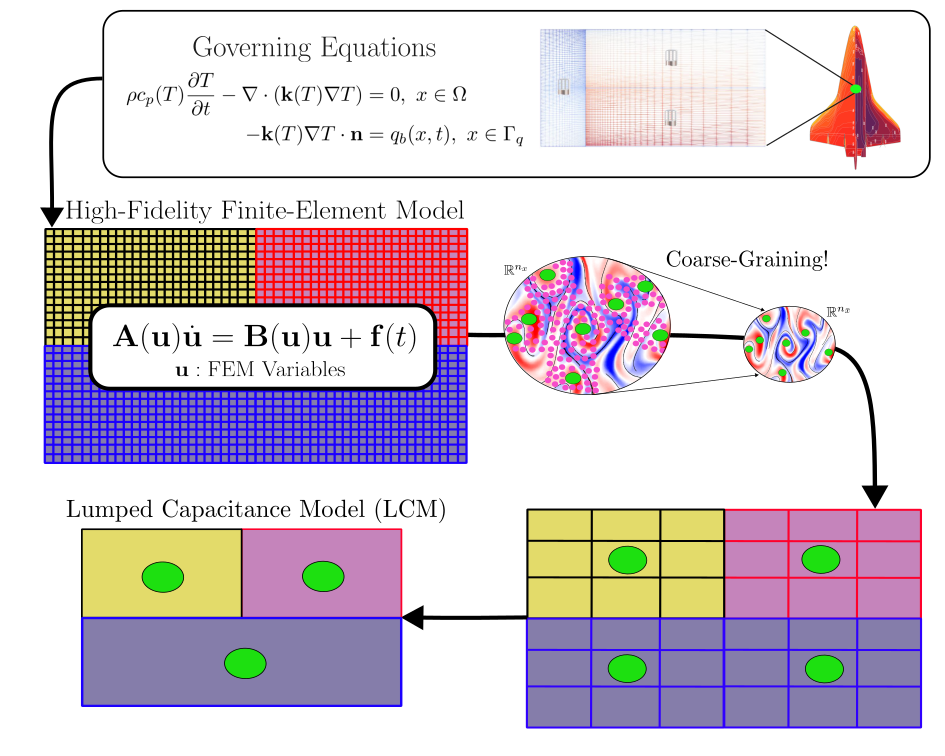
\includegraphics[width=0.85\textwidth]{../figs/pirom/coarse_graining_tps_left_4.png}
                \end{figure}}
        \end{column}}
        \hspace*{-0.25in}
        \visible<1->{
        \begin{column}{0.55\textwidth}
            \vspace*{-0.05in}
            \only<5>{
                \begin{figure}
                    \centering
                    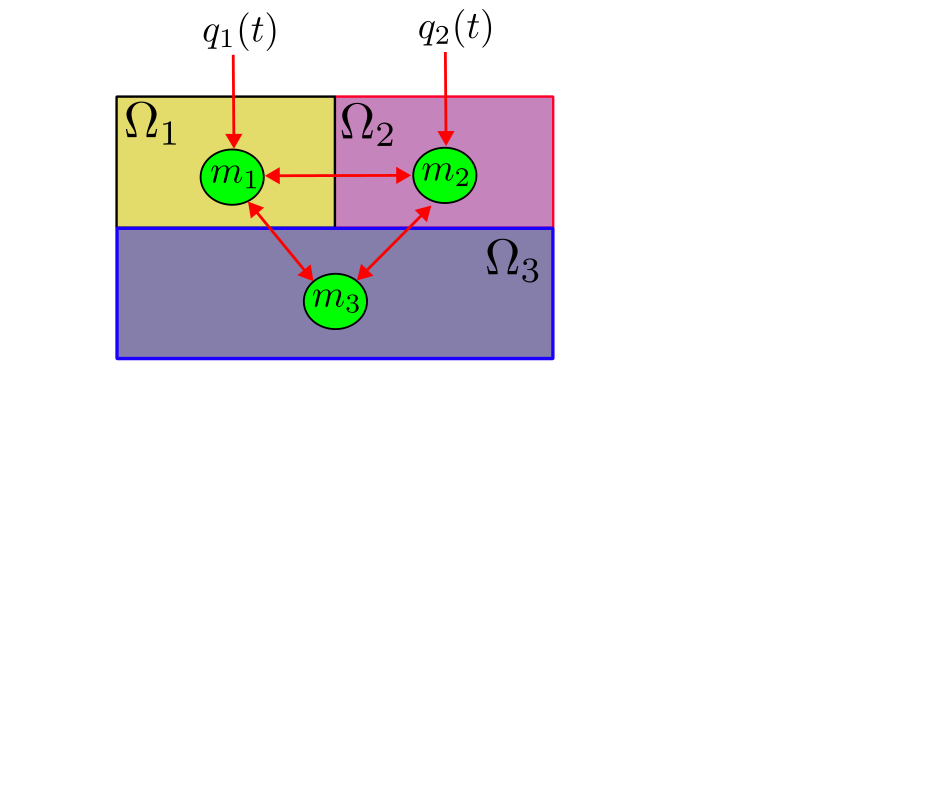
\includegraphics[width=0.95\textwidth]{../figs/pirom/coarse_grained_variables_tps_1.png}
                \end{figure}}
            \only<6>{
                \begin{figure}
                    \centering
                    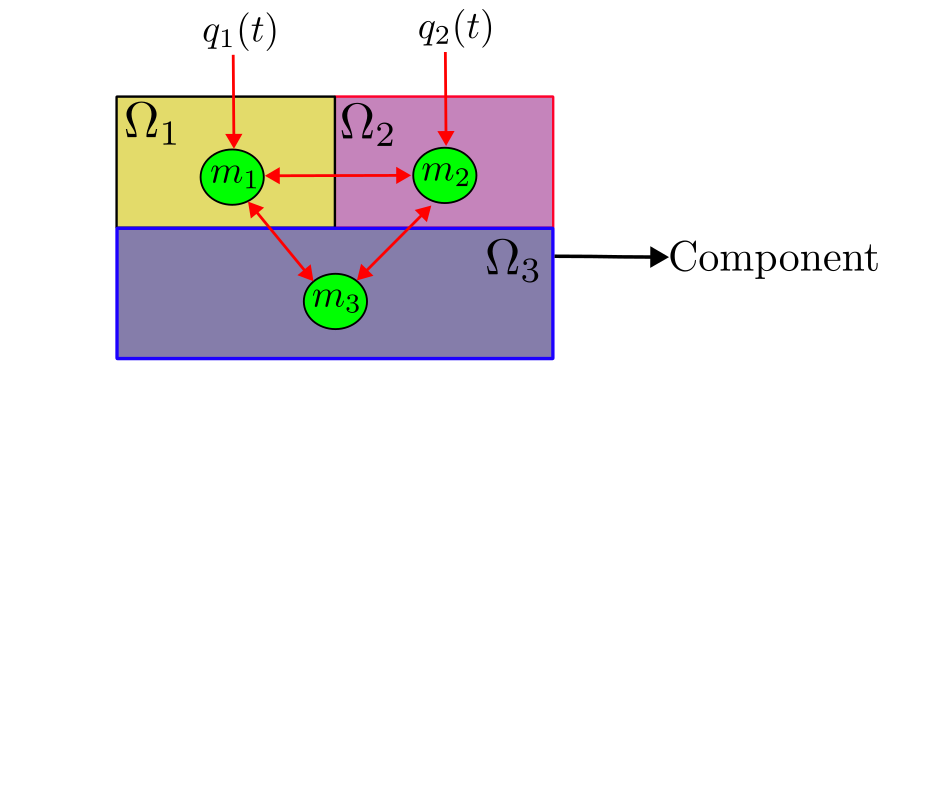
\includegraphics[width=0.95\textwidth]{../figs/pirom/coarse_grained_variables_tps_2.png}
                \end{figure}}
            \only<7>{
                \begin{figure}
                    \centering
                    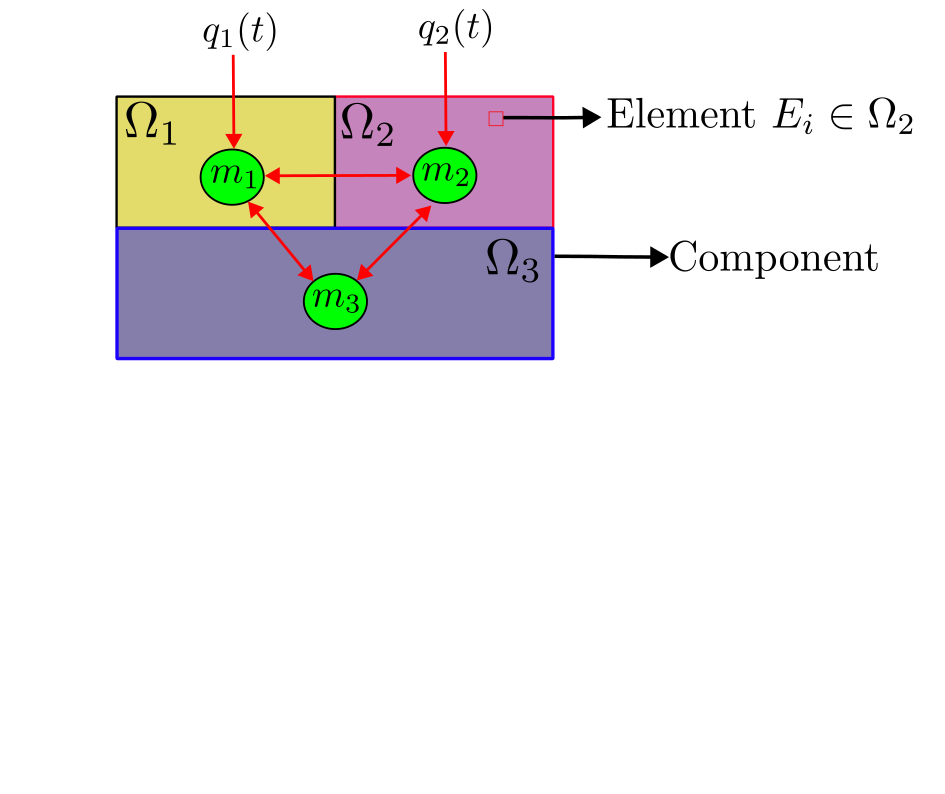
\includegraphics[width=0.95\textwidth]{../figs/pirom/coarse_grained_variables_tps_3.png}
                \end{figure}}
            \only<8>{
                \begin{figure}
                    \centering
                    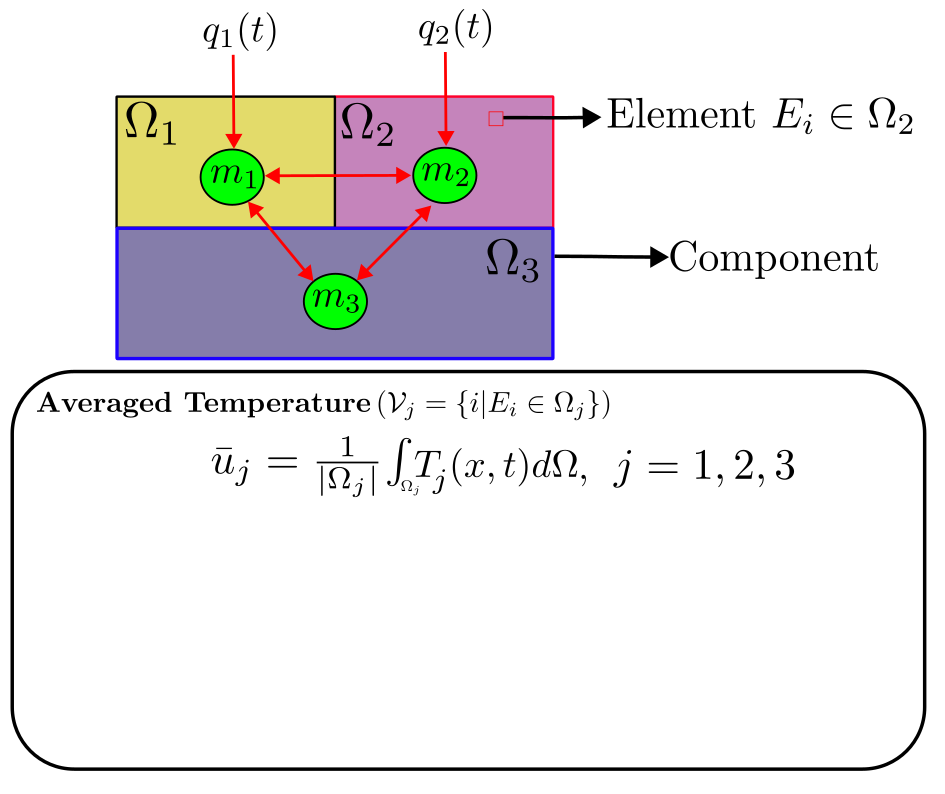
\includegraphics[width=0.95\textwidth]{../figs/pirom/coarse_grained_variables_tps_4.png}
                \end{figure}}
            \only<9>{
                \begin{figure}
                    \centering
                    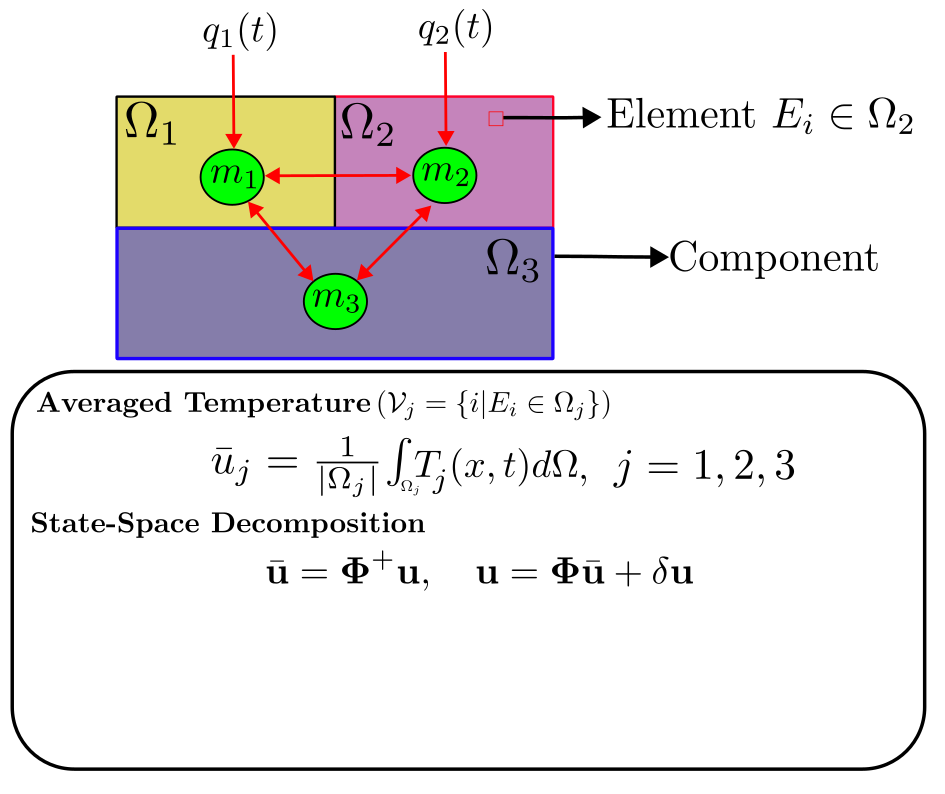
\includegraphics[width=0.95\textwidth]{../figs/pirom/coarse_grained_variables_tps_5.png}
                \end{figure}}
            \only<10>{
                \begin{figure}
                    \centering
                    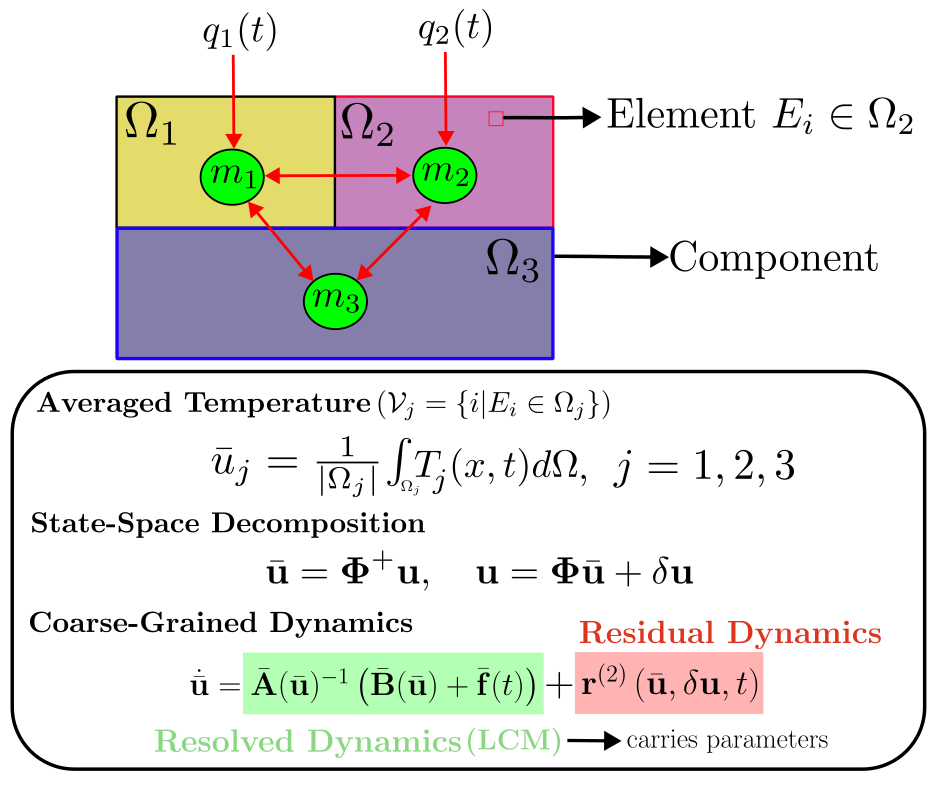
\includegraphics[width=0.95\textwidth]{../figs/pirom/coarse_grained_variables_tps_6.png}
                \end{figure}}
        \end{column}}
    \end{columns}
\end{frame}

\begin{frame}{Addressing the ITM: Physics Infusion}
    \footnotesize
    \visible<1->{
        Mori-Zwanzig (MZ) connects the \textbf{averaged} and \textbf{residual} dynamics for \textbf{physics-infusion} {\tiny [2]},}
    \visible<2->{
    \begin{equation*}
        \text{Projected GLE}:\quad \underbrace{\frac{\partial}{\partial t} \cP e^{t\cL}\bvu}_{\text{Observable Dynamics}} \visible<3->{= \underbrace{\cP e^{t\cL}\cP\cL\bvu}_{\text{Markovian}}} \visible<4->{+ \cP\underbrace{\int_0^t e^{(t-s)\cL}\cP\cL e^{s\cQ\cL}\cQ\cL\bvu ds}_{\text{Non-Markovian}}} \visible<5->{+ \cP\underbrace{e^{t\cQ\cL}\cQ\cL\bvu}_{\text{Noise}}}
    \end{equation*}}
    \begin{columns}
        \visible<3->{
        \begin{column}{0.3\textwidth}
            \centering
            \textbf{Markovian}
            \begin{figure}
                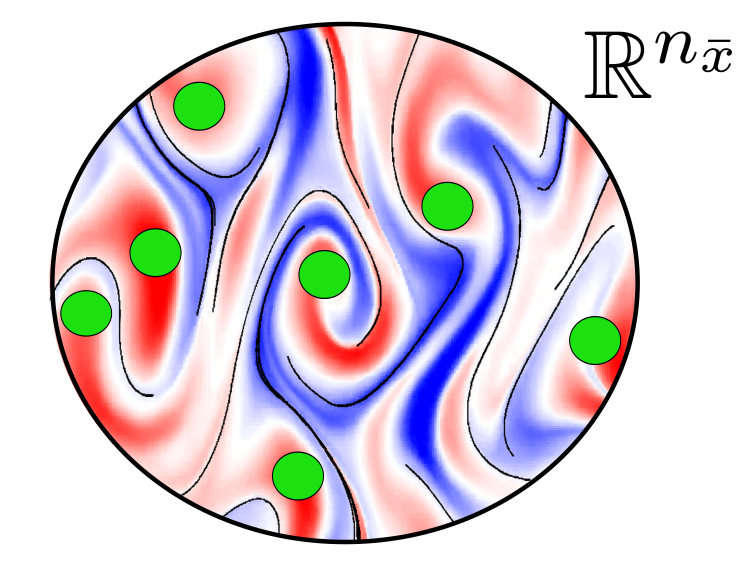
\includegraphics[width=0.9\textwidth]{../figs/pirom/coarse_variables.png}
            \end{figure}
            {\small (known dynamics)}
        \end{column}}
        \visible<4->{
        \begin{column}{0.3\textwidth}
            \centering
            \textbf{Non-Markovian}
            \begin{figure}
                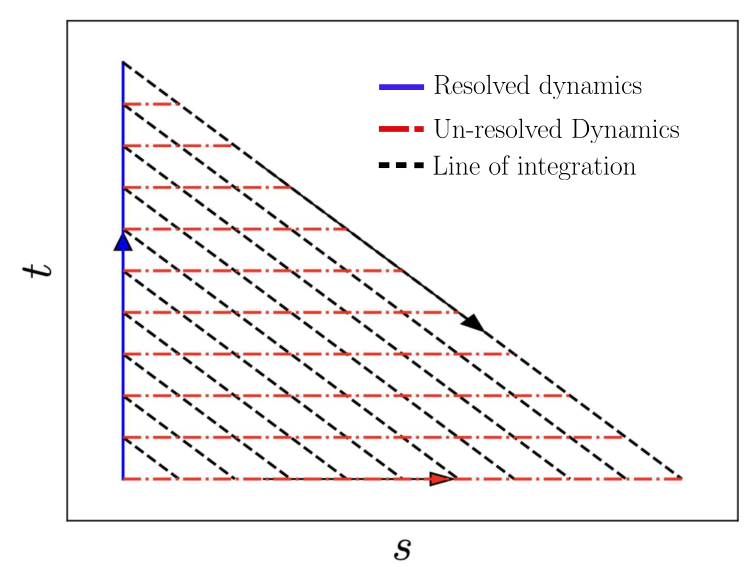
\includegraphics[width=0.9\textwidth]{../figs/pirom/memory.png}{\tiny [1]}
            \end{figure}
            {\small\textcolor{red}{(unknown dynamics)}}
        \end{column}}
        \visible<5->{
        \begin{column}{0.3\textwidth}
            \centering
            \textbf{Noise}
            \begin{figure}
                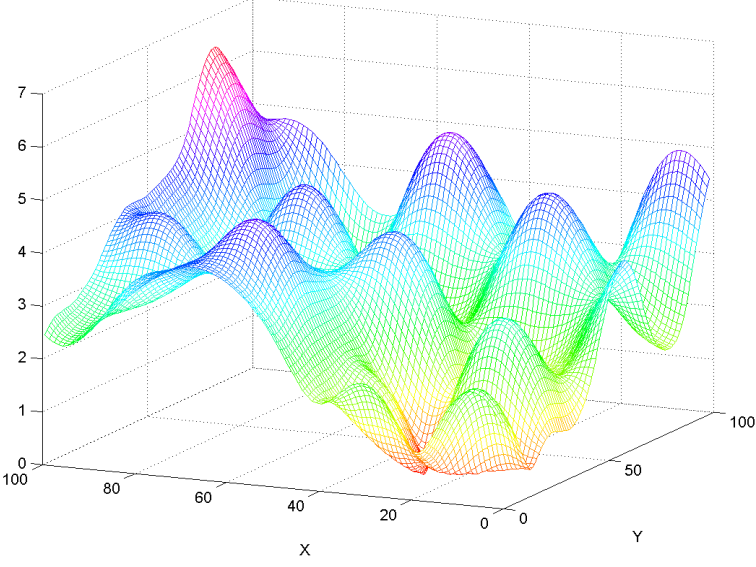
\includegraphics[width=0.9\textwidth]{../figs/pirom/noise.png}
            \end{figure}
            {\small\textcolor{black}{(orthogonal to $\cP$)}}
        \end{column}}
    \end{columns}
    \begin{center}
        {\tiny GLE: Generalized Langevin Equation, $\cL$: Liouville operator, PGLE: Projected GLE}
    \end{center}
\end{frame}

\begin{frame}{\large Approximate the Memory Kernel for Physics Infusion}
    \footnotesize
    \begin{columns}
        \begin{column}{0.5\textwidth}
            \visible<2->{
            \begin{graybox}{Memory Kernel Parametrization}
                \visible<3->{
                Define the memory kernel,
                \begin{equation*}
                    \vkappa(\bvu,t,s) = \cP e^{(t-s)\cL}\cP\cL e^{s\cQ\cL}\cQ\cL\bvu
                \end{equation*}}
                \visible<4->{
                Parametrize the \textbf{memory kernel},
                \vspace*{-0.05in}
                \begin{equation*}
                    \vkappa(\bvu,t,s;\redvTheta) \approx \sum_{j=1}^{m} \cK_j(t,s,\bvu;\redvTheta)\phi_j(s,\bvu;\redvTheta)
                \end{equation*}}
                \vspace*{-0.05in}
                \visible<5->{
                For \textbf{TPS problem}, design $\cK_j$ and $\phi_j$ as,
                \vspace*{-0.05in}
                \begin{align*}
                    \cK_j(t,s,\bvu;\redvTheta) &= e^{-\textcolor{red}{\lambda_j}(t-s)}\Rightarrow\text{{\tiny \textbf{exponential decay!}}}\\
                    \phi_j(s,\bvu;\redvTheta) &= \textcolor{red}{\vp_j}\left(\textcolor{red}{\vq_j}^\top\bar{\vu}(s) + \textcolor{red}{\vr_j}^\top\underbrace{\bar{\vf}(s)}_{\text{external forcing}} \right)
                \end{align*}}
            \end{graybox}}
        \end{column}
        \hspace*{-0.1in}
        \begin{column}{0.55\textwidth}
            \visible<6->{
            \begin{graybox}{Markovian Reformulation}
                \visible<7->{
                Define the \textbf{memory variables} as,
                \vspace*{-0.05in}
                \begin{equation*}
                    \beta_j(t) = \int_0^t e^{-\textcolor{red}{\lambda_j}(t-s)} \left(\textcolor{red}{\vq_j}^\top\bar{\vu}(s) + \textcolor{red}{\vr_j}^\top\bar{\vf}(s)\right) ds
                \end{equation*}}
                \visible<8->{
                so that the \textbf{hidden dynamics} are,
                \vspace*{-0.05in}
                \begin{equation*}
                    \dot{\beta}_j = \textcolor{red}{\lambda_j}\beta_j + \textcolor{red}{\vq_j}^\top\bar{\vu} + \textcolor{red}{\vr_j}^\top\bar{\vf},\:\: j=1,\dots,m
                \end{equation*}}
                \visible<9->{
                Thus, \textbf{the PIROM may be written as},
                \vspace*{-0.05in}
                \begin{align*}
                    \dot{\bvu} &= \underbrace{\cP e^{t\cL}\cP\cL\bvu}_{\text{\textbf{LCM dynamics!}}} + \sum_{j=1}^{m}\textcolor{red}{\vp_j}\beta_j\\
                    \vspace*{-0.01in}
                    \dot{\beta}_j &= \textcolor{red}{\lambda_j}\beta_j + \textcolor{red}{\vq_j}^\top\bar{\vu} + \textcolor{red}{\vr_j}^\top\bar{\vf}\\
                    \vspace*{-0.01in}
                    \vz &= \textcolor{red}{\vD_{\bar{u}}}\bvu + \textcolor{red}{\vD_{\beta}}\boldsymbol{\beta}
                    \vspace*{-0.05in}
                \end{align*}}
                \visible<10->{
                \vspace*{-0.05in}
                $\redvTheta = \left\{\textcolor{red}{\vP,\vQ,\vLambda,\vR,\vD_{\bar{u}},\vD_{\beta}}\right\}$ learnable parameters}
                \vspace*{0.05in}
            \end{graybox}}
        \end{column}
    \end{columns}
\end{frame}

\begin{frame}{\large Learning the Hidden Dynamics}
    \footnotesize
    \begin{columns}
        \begin{column}{0.6\textwidth}
            \centering
            \vspace*{-0.2in}
            \only<9>{
            \begin{figure}
                \centering
                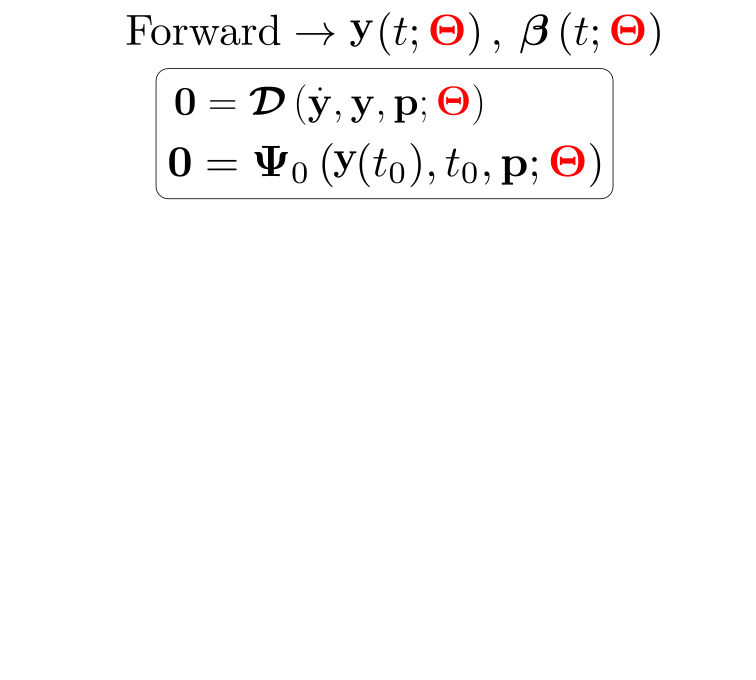
\includegraphics[width=0.7\textwidth]{../figs/pirom/adjoint_gradient_1.png}
            \end{figure}}
            \only<10>{
            \begin{figure}
                \centering
                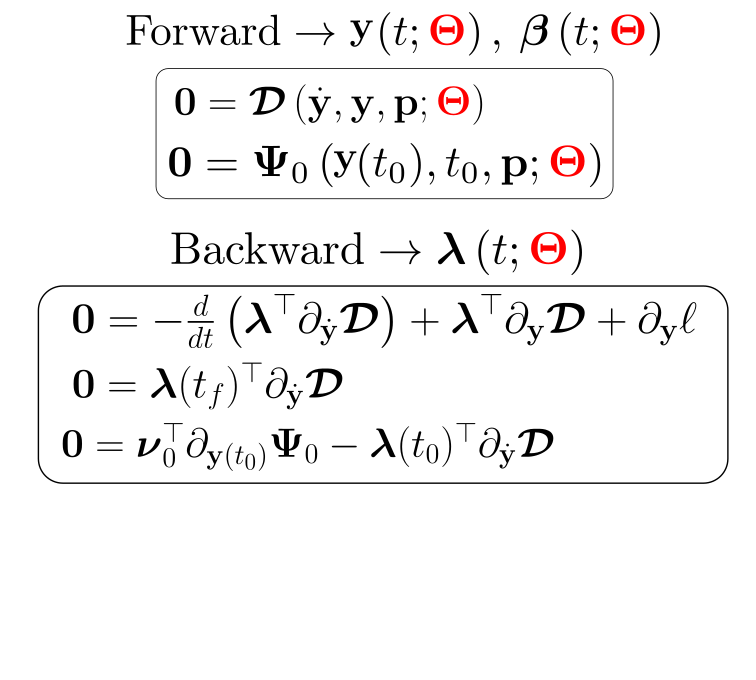
\includegraphics[width=0.7\textwidth]{../figs/pirom/adjoint_gradient_2.png}
            \end{figure}}
            \only<11>{
            \begin{figure}
                \centering
                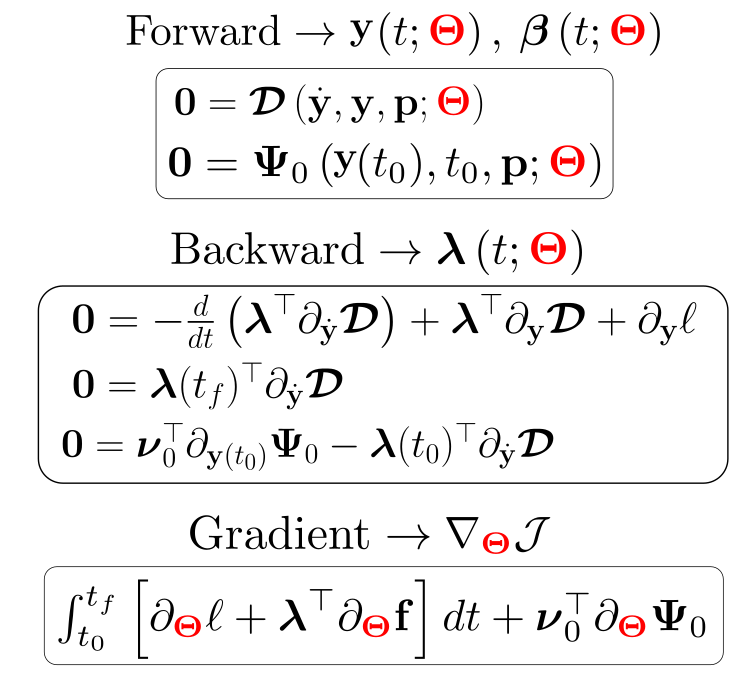
\includegraphics[width=0.7\textwidth]{../figs/pirom/adjoint_gradient_3.png}
            \end{figure}}
        \end{column}
        \hspace*{-0.5in}
        \begin{column}{0.45\textwidth}
            \visible<2->{
            \begin{graybox}{Constrained Parameter Opt.}
                \vspace*{-0.1in}
                \begin{align*}
                    \vspace*{0.05in}
                    \visible<3->{
                    \min_{\redvTheta} &\quad \cJ\left(\redvTheta\right) = \frac{1}{N} \sum_{l=1}^{N}\int_{t_0}^{t_f}\ell^{(l)}dt}\\
                    \visible<7->{
                    \text{s.t.} &\quad \vzero = \boldsymbol{\mathcal{D}}\left(\vy^{(l)},\dot{\vy}^{(l)},\vp^{(l)};\redvTheta\right)}\\
                    \visible<8->{
                    &\quad \boldsymbol{0} = \vPsi_0\left(\vy^{(l)}(t_0),t_0;\redvTheta\right)}
                \end{align*}
                \vspace*{-0.2in}
                \begin{itemize}
                    \item<4-> $\ell^{(l)} = \left\|\vz^{(l)} - \vz_{\text{HF}}^{(l)}\right\|_2^2$
                    \vspace*{-0.02in}
                    \item<5-> $\vz_{\text{HF}},\vz$ HF and PIROM observables,
                    \vspace*{-0.02in}
                    \item<6-> $\vy = \left[\bar{\vu},\vbeta\right]^\top$ PIROM state, 
                    \vspace*{-0.02in}
                    \item<7-> $\vcD$: PIROM compact dynamics,
                    \vspace*{-0.02in}
                    \item<8-> $\vPsi_0$: initial condition.
                    \vspace*{-0.1in}
                \end{itemize}
                \hspace*{-0.1in}
            \end{graybox}}
        \end{column}
    \end{columns}
\end{frame}